\documentclass[13pt, a4paper]{article}
\usepackage[utf8]{vietnam} 
\usepackage{amssymb,gensymb,textcomp} \usepackage{array,multicol,multirow,siunitx,tabularx}
\usepackage{graphicx} 
\usepackage{float}
\usepackage{multicol}
\usepackage{multirow}
\usepackage{adjustbox}
\usepackage{lipsum}
\usepackage{subcaption}
\usepackage{enumerate}
\usepackage{indentfirst}
\usepackage{amsmath} 
\usepackage{listings}
\usepackage{diagbox}
\usepackage{matlab-prettifier}
\usepackage{xcolor}
\usepackage{color}
\definecolor{light-gray}{gray}{0.95}
\newcommand{\code}[1]{\colorbox{light-gray}{\texttt{#1}}}
\usepackage{titlesec}
\usepackage{amsfonts} 
\usepackage{caption}
\usepackage{subcaption}
\usepackage{amssymb} 
\usepackage{rotating}
\usepackage{tikz}
\usepackage{verbatim}
\usepackage{subcaption}

\usepackage[colorlinks = true,
            linkcolor = black,
            urlcolor  = blue,
            citecolor = blue,
            anchorcolor = blue]{hyperref}
\usepackage{enumitem}
\usepackage[left=2.3cm,right=2cm,top=2.5cm,bottom=2.5cm]{geometry} 
\usepackage{scrextend}
\usepackage{algorithm2e}
\usepackage{etoolbox}
\usepackage{ragged2e}
\usepackage{minted}
\usepackage{lastpage}
\changefontsizes[23pt]{13pt}
\usepackage{fancyhdr}
\usepackage{tikz,tkz-tab}
\usetikzlibrary{shapes.geometric, arrows}
\usepackage[framemethod=TikZ]{mdframed}
\usepackage{amsthm}
\usepackage{xurl}
\usepackage{commath}
\usepackage{framed}
\usepackage{commath}
\usepackage{framed}
\usepackage{enumitem}
\usepackage{booktabs}
\makeatletter
\newcommand{\mylabel}[2]{#2\def\@currentlabel{#2}\label{#1}}
\makeatother

\renewcommand{\figureautorefname}{Hình}
\renewcommand{\tableautorefname}{Bảng}
\renewcommand{\equationautorefname}{Phương trình}
\renewcommand{\sectionautorefname}{Mục}
\renewcommand{\subsectionautorefname}{Phần}
\renewcommand{\subsubsectionautorefname}{Phần}
\renewcommand{\itemautorefname}{}
\renewcommand{\algorithmautorefname}{Thuật toán}
\setlength{\headheight}{20pt}
\captionsetup{labelfont={bf}}
\pagestyle{fancy}

\fancyhf{} % clear all header fields
\fancyhead[L]{
 \begin{tabular}{rl}
    \begin{picture}(15,15)(0,0)
    \put(0,-8){
\includegraphics[width=8.7mm, height=8.7mm]{SourceImage/LogoBK.png}}
   \end{picture}&
	\begin{tabular}{l}
		\textbf{\bf \ttfamily\color{blue}Trường Đại học Bách khoa - ĐHQG–HCM}
             \\[-1.4ex] \textbf{\bf \ttfamily\color{blue} Khoa Khoa học và Kỹ thuật Máy tính} 
	\end{tabular} 
 \end{tabular}
}
\fancyhead[R]{
 \begin{tabular}{r}
    \textbf{\bf \ttfamily \color{blue} Nhóm 023}
\end{tabular} 
}
\fancyfoot{} % clear all footer fields
\fancyfoot[L]{\footnotesize \ttfamily \textcolor{blue}{Internet of Things Assignment - HK241}}
\fancyfoot[R]{\footnotesize \ttfamily \textcolor{blue}{Trang {\thepage}/{\hypersetup{linkcolor=blue}\pageref{LastPage}}}}

\renewcommand{\footrulewidth}{1pt}
\definecolor{codegreen}{rgb}{0,0.6,0}
\definecolor{codegray}{rgb}{0.5,0.5,0.5}
\definecolor{codepurple}{rgb}{0.58,0,0.82}
\definecolor{backcolour}{rgb}{0.95,0.95,0.92}
\definecolor{bluehcmut}{RGB}{3, 43, 145}


\lstdefinestyle{mystyle}{
    language=R,% set programming language
    backgroundcolor=\color{backcolour},   
    commentstyle=\color{codegreen},
    keywordstyle=\color{blue},
    numberstyle=\tiny\color{codegray},
    stringstyle=\color{codepurple},
    basicstyle=\ttfamily\footnotesize,
    breakatwhitespace=false,         
    breaklines=true,
    captionpos=b,                    
    keepspaces=true,                 
    numbers=left,                    
    numbersep=5pt,
    frame = tb,
    showspaces=false,                
    showstringspaces=false,
    showtabs=false,                  
    tabsize=2
    escapeinside={(*}{*)},% escaping to LaTeX
    fancyvrb=true,% verbatim code is typset by listings
    extendedchars=false,% prohibit extended chars (chars of codes 128--255)
    alsoother={\$},% becomes other
    otherkeywords={!=, \~, \$, \&, \%/\%, \%*\%, \%\%, <-, <<-, /},% other keywords
    deletekeywords={c}% remove keywords
}
\lstset{
    backgroundcolor=\color{backcolour},   
    commentstyle=\color{codegreen},
    keywordstyle=\color{blue},
    numberstyle=\tiny\color{codegray},
    stringstyle=\color{codepurple},
    basicstyle=\ttfamily\footnotesize,
    breakatwhitespace=false,         
    breaklines=true,
    captionpos=b,                    
    keepspaces=true,                 
    numbers=left,                    
    numbersep=5pt,
    frame=tb,
    showspaces=false,                
    showstringspaces=false,
    showtabs=false,                  
    tabsize=4,
    columns=flexible
}

\usepackage{bashful}
\usepackage{tcolorbox}
\tcbuselibrary{minted,breakable,xparse,skins}
\definecolor{bg}{gray}{0.95}
\DeclareTCBListing{mintedbox}{O{}m!O{}}{%
  breakable=true,
  listing engine=minted,
  listing only,
  minted language=#2,
  minted style=default,
  minted options={%
    linenos=true,
    gobble=0,
    breaklines=true,
    breakafter=,,
    fontsize=\small,
    numbersep=8pt,
    #1},
  boxsep=0pt,
  left skip=0pt,
  right skip=0pt,
  left=25pt,
  right=0pt,
  top=3pt,
  bottom=3pt,
  arc=5pt,
  leftrule=0pt,
  rightrule=0pt,
  bottomrule=2pt,
  toprule=2pt,
  colframe=orange!70,
  enhanced,
  overlay={%
    \begin{tcbclipinterior}
    \fill[orange!20!white] (frame.south west) rectangle ([xshift=20pt]frame.north west);
    \end{tcbclipinterior}},
  #3}

\makeatletter
\AtBeginEnvironment{mintedbox}{\dontdofcolorbox}
\def\dontdofcolorbox{\renewcommand\fcolorbox[4][]{##4}}
\makeatother

\setcounter{secnumdepth}{4}

\titleformat{\paragraph}
{\normalfont\normalsize\itshape}{\theparagraph}{1em}{}
\titlespacing*{\paragraph}
{0pt}{3.25ex plus 1ex minus .2ex}{1.5ex plus .2ex}


\titleformat{\listing}
{\normalfont\normalsize\itshape}{\theparagraph}{1em}{}
\titlespacing*{\listing}
{0pt}{3.25ex plus 1ex minus .2ex}{1.5ex plus .2ex}

\begin{document}
%\begin{comment}
\setlength{\textfloatsep}{1.5pt} % Đặt khoảng cách giữa các figure

\begin{titlepage}
\begin{tikzpicture}[remember picture,overlay,inner sep=0,outer sep=0]
     \draw[blue!70!black,line width=4pt] ([xshift=-1.5cm,yshift=-2cm]current page.north east) coordinate (A)--([xshift=1.5cm,yshift=-2cm]current page.north west) coordinate(B)--([xshift=1.5cm,yshift=2cm]current page.south west) coordinate (C)--([xshift=-1.5cm,yshift=2cm]current page.south east) coordinate(D)--cycle;

     \draw ([yshift=0.5cm,xshift=-0.5cm]A)-- ([yshift=0.5cm,xshift=0.5cm]B)--
     ([yshift=-0.5cm,xshift=0.5cm]B) --([yshift=-0.5cm,xshift=-0.5cm]B)--([yshift=0.5cm,xshift=-0.5cm]C)--([yshift=0.5cm,xshift=0.5cm]C)--([yshift=-0.5cm,xshift=0.5cm]C)-- ([yshift=-0.5cm,xshift=-0.5cm]D)--([yshift=0.5cm,xshift=-0.5cm]D)--([yshift=0.5cm,xshift=0.5cm]D)--([yshift=-0.5cm,xshift=0.5cm]A)--([yshift=-0.5cm,xshift=-0.5cm]A)--([yshift=0.5cm,xshift=-0.5cm]A);


     \draw ([yshift=-0.3cm,xshift=0.3cm]A)-- ([yshift=-0.3cm,xshift=-0.3cm]B)--
     ([yshift=0.3cm,xshift=-0.3cm]B) --([yshift=0.3cm,xshift=0.3cm]B)--([yshift=-0.3cm,xshift=0.3cm]C)--([yshift=-0.3cm,xshift=-0.3cm]C)--([yshift=0.3cm,xshift=-0.3cm]C)-- ([yshift=0.3cm,xshift=0.3cm]D)--([yshift=-0.3cm,xshift=0.3cm]D)--([yshift=-0.3cm,xshift=-0.3cm]D)--([yshift=0.3cm,xshift=-0.3cm]A)--([yshift=0.3cm,xshift=0.3cm]A)--([yshift=-0.3cm,xshift=0.3cm]A);

   \end{tikzpicture}
\begin{center}
    \vspace{-10pt}
    \textbf{ĐẠI HỌC QUỐC GIA THÀNH PHỐ HỒ CHÍ MINH}\\
    \textbf{TRƯỜNG ĐẠI HỌC BÁCH KHOA}\\
    \textbf{KHOA KHOA HỌC VÀ KỸ THUẬT MÁY TÍNH}\\
    \vspace{10pt}
    
\includegraphics[width=0.35\linewidth]{SourceImage/LogoBK.png}\\
    \vspace{10pt}
    \textbf{\Large BÀI TẬP LỚN}\\
    \vspace{8pt}
    \textbf{\Large PHÁT TRIỂN ỨNG DỤNG INTERNET OF THINGS (CO3037)}\\
    \vspace{30pt}
    \hrule
    \vspace{16pt}
    \textcolor{bluehcmut}{\LARGE{\textbf{Internet of Things Project Assignment}}}\\
    \vspace{16pt}
    \hrule
\end{center}
\begin{center}
    \textbf{Giảng viên hướng dẫn:  Lê Trọng Nhân}\\
    \textbf{HK252}\\
\end{center}
\vspace{10pt}
\vspace{-.2cm}
\begin{adjustbox}{width=0.94\textwidth,center=\textwidth}
    \small
    \begin{tabular}{|>{\centering\arraybackslash}m{0.8cm}|>{\centering\arraybackslash}m{5.0cm}|>{\centering\arraybackslash}m{1.6cm}|>{\centering\arraybackslash}m{1.2cm}|>{\centering\arraybackslash}m{4.0cm}|}
        \hline
        \textbf{STT} & \textbf{Họ và tên} & \textbf{MSSV} & \textbf{Lớp} & \textbf{Ghi chú}\\
        \hline
        \textbf{1} & \textbf{Hồ Đăng Khoa} & \textbf{2211588} & \textbf{L01} & \textbf{Nhóm trưởng}\\
        \hline
        2 & Hoàng Sỹ Xuân Sơn & 2212937 & L01 &  \\
        \hline
        3 & Vũ Đức Lâm & 2211824 & L01 &  \\
        \hline
        4 & Nguyễn Minh Hưng & 2211367 & L01 & \\
        \hline
    \end{tabular}
\end{adjustbox}

\begin{center}
    ~\\
    ~\\
    \textit{Thành phố Hồ Chí Minh, tháng 5 năm 2026}
\end{center}
\end{titlepage}
\begin{titlepage}
    \section*{Danh sách thành viên}
    \begin{adjustbox}{width=1.08\textwidth,center=\textwidth}
    \small
        \begin{tabular}{|>{\centering\arraybackslash}m{0.8cm}|>{\centering\arraybackslash}m{4cm}|>{\centering\arraybackslash}m{1.5cm}|>{\centering\arraybackslash}m{5.8cm}|>{\centering\arraybackslash}m{2.05cm}|}
            \hline
            \textbf{STT} & \textbf{Họ và tên} & \textbf{MSSV} & \textbf{Nhiệm vụ} & \textbf{Đóng góp}\\
            \hline
            1 & Hồ Đăng Khoa & 2211588 &  & 100\% 
            \\
            \hline
           2 & Hoàng Sỹ Xuân Sơn	 & 2212937 & & 100\% 
            \\
            \hline
           3 & Vũ Đức Lâm & 2212466 & & 100\% 
            \\
            \hline
            4 & Nguyễn Minh Hưng & 2211367 &  & 100 \% & 
            \\
        \hline
        \end{tabular}
    \end{adjustbox}
\end{titlepage}
% \begin{titlepage}
    \section*{Danh sách từ viết tắt}
    \begin{adjustbox}{width=1.08\textwidth,center=\textwidth}
    \small
        \begin{tabular}{|>{\centering\arraybackslash}m{0.8cm}|>{\centering\arraybackslash}m{3cm}|>{\raggedright\arraybackslash}m{6cm}|>
        {\raggedright\arraybackslash}m{6cm}|}
            \hline
            \textbf{STT} & \textbf{Từ viết tắt} & \textbf{Từ đầy đủ} & \textbf{Ý nghĩa}  \\
            \hline
            1 & BPP & Bin Packing Problem & Bài toán đóng thùng    \\
            \hline
            2 & 2DCSP & The Two-dimension Cutting-Stock Problem & Bài toán cắt vật liệu hai chiều  \\
            \hline
           3 & 2DVSBPP & The Two-dimension Variable-Sized Bin Packing Problem & Bài toán đóng thùng hai chiều có kích thước thùng thay đổi \\
            \hline
           4& C\&P  &  Cutting and Packing  & Cắt và đóng gói          \\
           \hline
            5&ILP& Integer Linear Programming  & Quy hoạch tuyến tính nguyên\\
            \hline
        \end{tabular}
    \end{adjustbox}
\end{titlepage}
% \newpage
% {%
% \let\oldnumberline\numberline%
% \renewcommand{\numberline}{\figurename~\oldnumberline}%
% \listofalgorithms%
% }
% \newpage
% % Định nghĩa lại cách hiển thị tên trong danh sách bảng
% {%
% \let\oldnumberline\numberline
% \renewcommand{\numberline}{\tablename~\oldnumberline}
% \listoftables
% }
% \newpage
\tableofcontents
\newpage 

\section{Giới thiệu}

Sự phát triển mạnh mẽ của Internet vạn vật (Internet of Things --- IoT) đặt ra yêu cầu ngày càng cao đối với các hệ thống nhúng về khả năng xử lý đa tác vụ, độ tin cậy theo thời gian thực và khả năng tích hợp với hạ tầng đám mây.
Báo cáo này trình bày quá trình thiết kế, triển khai và đánh giá một hệ thống nhúng thời gian thực hoàn chỉnh trên nền tảng vi điều khiển ESP32-S3 (bo mạch Yolo UNO), sử dụng hệ điều hành thời gian thực FreeRTOS~\cite{freertos} làm nền tảng điều phối tác vụ.
Dự án được xây dựng dựa trên mã nguồn gốc YoloUNO PlatformIO RTOS\_Project~\cite{yolouno} và mở rộng với các chức năng khác biệt ít nhất 30\% so với mã nguồn gốc, bao gồm kiến trúc đồng bộ hóa không có biến toàn cục, giao diện giám sát Web theo thời gian thực, suy luận máy học tại biên (TinyML) và tích hợp nền tảng đám mây CoreIOT~\cite{coreiot}.

\subsection{Mục tiêu của hệ thống}

Mục tiêu tổng quát của đề tài là phát triển một hệ thống giám sát môi trường và điều khiển thiết bị ngoại vi hoàn chỉnh trên vi điều khiển ESP32-S3, đảm bảo toàn bộ việc chia sẻ dữ liệu giữa các tác vụ được thực hiện thông qua các cơ chế đồng bộ hóa của FreeRTOS (Mutex và Binary Semaphore) mà không sử dụng bất kỳ biến toàn cục nào.
Cụ thể, hệ thống cần hoàn thành sáu nhiệm vụ độc lập nhưng được tích hợp chặt chẽ với nhau như sau:

\begin{itemize}
    \item \textbf{Nhiệm vụ 1: Đèn LED đơn nhấp nháy theo điều kiện nhiệt độ.}
    Xác định lại chế độ nhấp nháy của đèn LED onboard (GPIO~38) để phản ứng với ít nhất ba khoảng nhiệt độ khác nhau, mỗi khoảng tương ứng với một tần số nhấp nháy riêng biệt.
    Cơ chế Binary Semaphore (\texttt{xLedSemaphore}) được sử dụng để đồng bộ hóa giữa tác vụ đọc cảm biến và tác vụ điều khiển LED, đảm bảo tính nhất quán của dữ liệu nhiệt độ trong môi trường đa tác vụ.

    \item \textbf{Nhiệm vụ 2: Điều khiển đèn LED NeoPixel theo độ ẩm.}
    Thiết kế lại các mẫu màu của đèn NeoPixel WS2812B onboard (GPIO~18) để biểu thị ít nhất ba mức độ ẩm khác nhau, với sự tương quan rõ ràng giữa từng khoảng giá trị độ ẩm và màu sắc hiển thị tương ứng.
    Kỹ thuật Binary Semaphore (\texttt{xNeoSemaphore}) được áp dụng để đồng bộ hóa quá trình cập nhật màu sắc giữa tác vụ cảm biến và tác vụ điều khiển NeoPixel.

    \item \textbf{Nhiệm vụ 3: Giám sát nhiệt độ và độ ẩm qua màn hình LCD.}
    Định nghĩa các điều kiện ngưỡng để tạo và giải phóng Mutex bảo vệ tài nguyên màn hình LCD 1602 I2C, hiển thị ít nhất ba trạng thái cảnh báo khác biệt (Normal, Warning, Critical) dựa trên giá trị đọc từ cảm biến DHT20~\cite{dht20}.
    Nhiệm vụ này cũng yêu cầu loại bỏ hoàn toàn tất cả biến toàn cục trong toàn bộ dự án, thay thế bằng cấu trúc dữ liệu dùng chung \texttt{SystemData} được bảo vệ bởi Mutex (\texttt{xMutex}).

    \item \textbf{Nhiệm vụ 4: Máy chủ Web ở chế độ điểm truy cập.}
    Thiết kế lại giao diện máy chủ web nhúng (\texttt{ESPAsyncWebServer}~\cite{espassyncwebserver}) để nâng cao khả năng sử dụng, kết hợp giao thức WebSocket (\texttt{/ws}) cho phép cập nhật dữ liệu cảm biến theo thời gian thực mà không cần tải lại trang.
    Giao diện phải bao gồm ít nhất hai nút điều khiển có nhãn rõ ràng để điều khiển độc lập hai thiết bị ngoại vi; toàn bộ tài nguyên giao diện được lưu trữ trên phân vùng LittleFS~\cite{littlefs} của bộ nhớ Flash.

    \item \textbf{Nhiệm vụ 5: Triển khai TinyML và đánh giá độ chính xác.}
    Mô tả tập dữ liệu huấn luyện bao gồm quá trình thu thập và gán nhãn dữ liệu, huấn luyện mạng nơ-ron phân loại và chuyển đổi sang định dạng C-array để nhúng trực tiếp vào chip.
    Mô hình được thực thi bằng thư viện TensorFlow Lite Micro~\cite{tflitemicro} trên Tensor Arena tĩnh 8~kB, với quá trình đo lường và đánh giá độ chính xác nhận dạng (Accuracy, Precision, Recall) trên tập kiểm thử, kèm thảo luận về hiệu suất và giới hạn của mô hình khi chạy trên phần cứng thực.

    \item \textbf{Nhiệm vụ 6: Xuất bản dữ liệu lên máy chủ đám mây CoreIOT.}
    Cấu hình ESP32-S3 ở chế độ Trạm (STA Mode) để thiết lập kết nối MQTT đến máy chủ CoreIOT~\cite{coreiot}, định kỳ xuất bản dữ liệu viễn trắc nhiệt độ và độ ẩm cùng thuộc tính định danh thiết bị (địa chỉ MAC).
    Thiết bị sử dụng mã xác thực (Device Token) hợp lệ khớp với thiết bị đã đăng ký trên nền tảng, tuân theo mẫu giải pháp chính thức của CoreIOT và thư viện ThingsBoard MQTT~\cite{thingsboard_mqtt}.
\end{itemize}

\subsection{Phạm vi và giới hạn}

Dự án được triển khai toàn bộ trên nền tảng vi điều khiển ESP32-S3 (bo mạch Yolo UNO) bằng ngôn ngữ C/C++ thông qua plugin PlatformIO~\cite{platformio}. Trong giới hạn của đề tài, cấu hình phần cứng của bo mạch được cố định ở chế độ 301B9 và 812H6.

Về mặt phần cứng, hệ thống sử dụng cảm biến DHT20~\cite{dht20} kết nối qua giao thức I2C (SDA: GPIO~11, SCL: GPIO~12) để thu thập nhiệt độ và độ ẩm, cùng các thiết bị ngoại vi onboard gồm LED đơn (GPIO~38), NeoPixel WS2812B~\cite{ws2812b} (GPIO~18) và màn hình LCD 1602 I2C.
Về mặt kết nối, hệ thống giới hạn ở giao tiếp Wi-Fi 2.4~GHz với một mạng nội bộ duy nhất.
Quá trình huấn luyện mô hình TinyML sử dụng tập dữ liệu có quy mô nhỏ, phù hợp với dung lượng RAM tĩnh 8~kB Tensor Arena của ESP32-S3, và nền tảng CoreIOT được sử dụng như giải pháp lưu trữ đám mây duy nhất thông qua thư viện ThingsBoard MQTT~\cite{thingsboard_mqtt}.
Việc kiểm thử hệ thống được thực hiện trong môi trường phòng thí nghiệm, tập trung vào tính đúng đắn của logic đồng bộ hóa đa tác vụ RTOS thay vì tối ưu hóa cho điều kiện vận hành khắc nghiệt ngoài trời.

\section{Cơ sở lý thuyết}

\subsection{Phần cứng}

\subsubsection{Bo mạch lập trình nhúng Yolo UNO và Vi điều khiển ESP32-S3}
Yolo UNO là một board mạch lập trình nhúng được thiết kế và phát triển nhằm phục vụ việc nghiên cứu, thử nghiệm và triển khai các ứng dụng kết nối vạn vật IoT và Trí tuệ nhân tạo (AI). Board mạch được xây dựng trên nền tảng vi điều khiển SoC dòng ESP32-S3 mã hiệu ESP32-S3-WROOM-1, sở hữu bộ xử lý lõi kép Xtensa 32-bit với tốc độ xung nhịp lên tới 240MHz. Bo mạch tích hợp sẵn 16~MB Flash và 8~MB PSRAM, đủ cho các ứng dụng đa nhiệm thời gian thực và suy luận TinyML.

Bo mạch hỗ trợ đồng thời hai chế độ kết nối không dây 2.4GHz Wi-Fi (chuẩn 802.11 b/g/n) và Bluetooth 5 (BLE), tích hợp sẵn 12 cổng kết nối chuẩn Grove mở rộng phân tách rõ ràng thành các cổng Analog, Digital và I2C, hỗ trợ kết nối nhiều loại cảm biến và ngoại vi. Trong dự án này, bo mạch được cấu hình hoạt động đồng bộ ở các chế độ phần cứng chuyên dụng 301B9 và 812H6.

\begin{figure}[H]
    \centering
    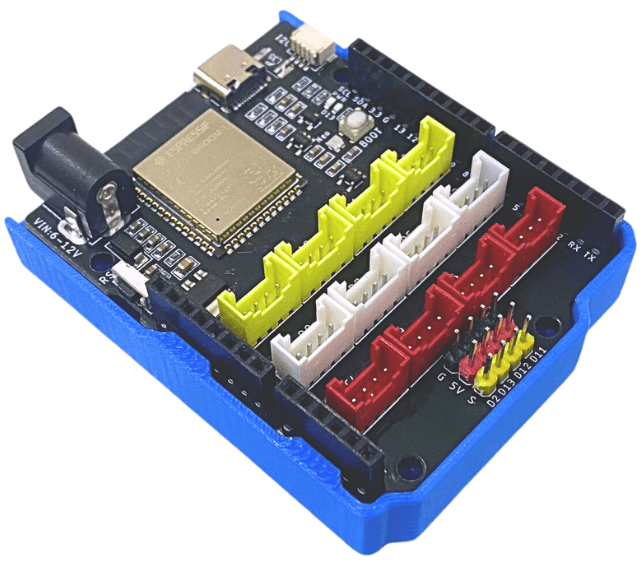
\includegraphics[width=0.5\textwidth]{SourceImage/yolo-uno.png}
    \caption{Board lập trình Yolo UNO và chip xử lý ESP32-S3}
    \label{fig:yolo_uno_board}
\end{figure}

\begin{table}[H]
    \centering
    \caption{Thông số kỹ thuật của board lập trình Yolo UNO trong hệ thống}
    \begin{tabular}{|l|l|}
    \hline
    \textbf{Thông số} & \textbf{Chi tiết} \\ \hline
    Vi xử lý & ESP32-S3 Dual Core 240MHz Tensilica Xtensa \\ \hline
    Bộ nhớ mở rộng & 16MB Flash, 8MB PSRAM \\ \hline
    Kết nối không dây & 2.4GHz Wi-Fi (802.11 b/g/n), Bluetooth 5.0, BLE \\ \hline
    Nguồn cấp hoạt động & 5VDC qua cổng USB Type-C hoặc Jack DC 5521 \\ \hline
    Nút nhấn tích hợp & Phím Reset, Phím chế độ Bootloader (BOOT0) \\ \hline
    Giao tiếp mở rộng & 12 cổng Grove (4 × Analog, 4 × Digital, 4 × I2C) \\ \hline
    Đèn hiển thị onboard & LED nguồn, LED chân D13, bóng LED RGB NeoPixel \\ \hline
    Chế độ cấu hình & Thiết lập chuẩn phần cứng 301B9 và 812H6 \\ \hline
    \end{tabular}
\end{table}

\subsubsection{Cảm biến nhiệt độ và độ ẩm DHT20}
DHT20 là dòng cảm biến nhiệt độ và độ ẩm kỹ thuật số thế hệ mới, được nâng cấp đáng kể so với các thế hệ trước. Cảm biến tích hợp chip ASIC cùng phần tử đo độ ẩm điện dung và đo nhiệt độ. DHT20 giao tiếp qua I2C, cho phép kết nối chung bus với các thiết bị I2C khác trên cùng bo mạch.

\begin{figure}[H]
    \centering
    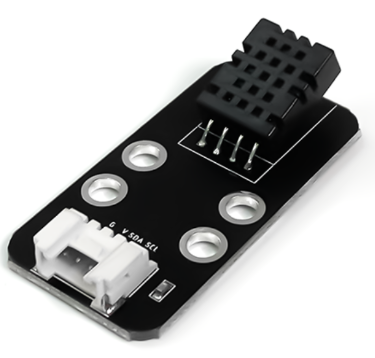
\includegraphics[width=0.4\textwidth]{SourceImage/DHT20 (1).png}
    \caption{Cảm biến nhiệt độ và độ ẩm kỹ thuật số I2C DHT20}
    \label{fig:sensor_dht20}
\end{figure}

\begin{table}[H]
    \centering
    \caption{Thông số kỹ thuật của cảm biến nhiệt độ và độ ẩm DHT20}
    \begin{tabular}{|l|l|}
    \hline
    \textbf{Thông số} & \textbf{Giá trị} \\ \hline
    Điện áp hoạt động & 2.2V -- 5.5V DC \\ \hline
    Giao thức truyền dữ liệu & I2C \\ \hline
    Phạm vi đo độ ẩm & 0\% -- 100\% RH \\ \hline
    Phạm vi đo nhiệt độ & -40$^{\circ}$C -- 80$^{\circ}$C \\ \hline
    Độ chính xác độ ẩm & $\pm$3\% RH \\ \hline
    Độ chính xác nhiệt độ & $\pm$0.5$^{\circ}$C \\ \hline
    \end{tabular}
\end{table}

\begin{table}[H]
    \centering
    \caption{Chức năng các chân kết nối của cảm biến DHT20}
    \begin{tabular}{|c|l|l|}
    \hline
    \textbf{STT} & \textbf{Chân} & \textbf{Chức năng} \\ \hline
    1 & VDD & Cấp nguồn dương (2.2V -- 5.5V) \\ \hline
    2 & SDA & Dây truyền nhận dữ liệu nối tiếp (Serial Data) \\ \hline
    3 & GND & Nối đất \\ \hline
    4 & SCL & Dây cấp xung nhịp nối tiếp (Serial Clock) \\ \hline
    \end{tabular}
\end{table}

\subsubsection{Đèn LED đơn cảnh báo (Tích hợp onboard)}
Trong dự án này, LED đơn được tích hợp sẵn trên bo mạch Yolo UNO, kết nối với GPIO~38. Binary Semaphore điều phối tần số nhấp nháy theo ba ngưỡng nhiệt độ.

\begin{table}[H]
    \centering
    \caption{Thông số kỹ thuật tiêu chuẩn của LED đơn cảnh báo}
    \begin{tabular}{|l|l|}
    \hline
    \textbf{Thông số} & \textbf{Giá trị} \\ \hline
    Điện áp kích hoạt thuận & 1.8V -- 2.2VDC (tùy thuộc màu sắc LED) \\ \hline
    Dòng điện hoạt động định mức & 10mA -- 20mA \\ \hline
    Dạng tín hiệu điều khiển & Kích hoạt mức logic (High/Low) hoặc xung PWM \\ \hline
    \end{tabular}
\end{table}

\subsubsection{Đèn LED màu NeoPixel WS2812B (Tích hợp onboard)}
NeoPixel WS2812B là LED RGB tích hợp chip điều khiển bên trong, cho phép điều khiển màu sắc từng pixel qua một dây tín hiệu số. Mỗi pixel nhận gói dữ liệu 24-bit, 8-bit cho mỗi kênh màu. NeoPixel cũng được tích hợp sẵn trên bo mạch Yolo UNO (GPIO~18), được dùng để hiển thị ba mức màu cảnh báo theo độ ẩm.

\begin{table}[H]
    \centering
    \caption{Thông số kỹ thuật của bóng LED màu NeoPixel onboard}
    \begin{tabular}{|l|l|}
    \hline
    \textbf{Thông số} & \textbf{Giá trị} \\ \hline
    Điện áp hoạt động cấp vào & 5VDC \\ \hline
    Kiểu IC điều khiển tích hợp & WS2812B \\ \hline
    Định dạng cấu trúc màu sắc & RGB 24-bit (16,7 triệu màu sắc) \\ \hline
    Tần số truyền nhận dữ liệu số & 800 Khz \\ \hline
    \end{tabular}
\end{table}

\subsubsection{Màn hình hiển thị LCD I2C}
Màn hình LCD 16$\times$2 hiển thị văn bản cục bộ trực tiếp trên thiết bị. Màn hình sử dụng giao tiếp I2C và kết nối vào cổng Grove I2C trên Yolo UNO qua cáp kết nối bốn dây (VCC, GND, SDA, SCL). Truy cập LCD được bảo vệ bằng Mutex để tránh xung đột bus I2C giữa các tác vụ, đồng thời hiển thị ba trạng thái cảnh báo.
\begin{figure}[H]
    \centering
    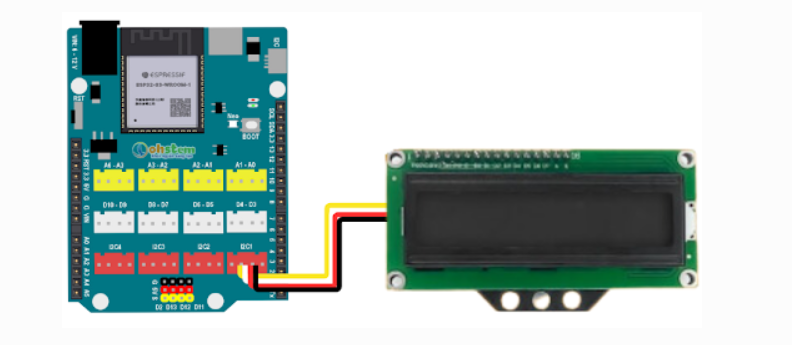
\includegraphics[width=0.9\textwidth]{SourceImage/LCD.png}
    \caption{Màn hình hiển thị LCD I2C cắm trực tiếp vào Yolo UNO qua cáp Grove}
    \label{fig:lcd_i2c}
\end{figure}
\begin{table}[H]
    \centering
    \caption{Thông số kỹ thuật của màn hình hiển thị LCD I2C}
    \begin{tabular}{|l|l|}
    \hline
    \textbf{Thông số} & \textbf{Giá trị} \\ \hline
    Điện áp hoạt động cấp vào & 5VDC \\ \hline
    Giao thức truyền dữ liệu chính & I2C \\ \hline
    Kết nối vật lý & Cáp 4 chân Grove (VCC, GND, SDA, SCL) \\ \hline
    Địa chỉ I2C mặc định & 0x27 hoặc 0x3F \\ \hline
    Đèn nền & Đèn LED tích hợp điều khiển qua phần mềm \\ \hline
    \end{tabular}
\end{table}
\begin{table}[H]
    \centering
    \caption{Chức năng các chân giao tiếp của màn hình LCD I2C}
    \begin{tabular}{|c|l|l|}
    \hline
    \textbf{STT} & \textbf{Chân} & \textbf{Chức năng} \\ \hline
    1 & GND & Nối đất \\ \hline
    2 & VCC & Cấp nguồn dương 5VDC \\ \hline
    3 & SDA & Dây truyền nhận dữ liệu nối tiếp (Serial Data) \\ \hline
    4 & SCL & Dây cấp xung nhịp nối tiếp (Serial Clock) \\ \hline
    \end{tabular}
\end{table}

\subsubsection{Giao thức truyền thông và kết nối}
Hệ thống IoT đòi hỏi sự linh hoạt trong cả truyền thông cục bộ cận biên lẫn truyền thông diện rộng lên máy chủ Internet:
\begin{itemize}
    \item \textbf{I2C:} Giao thức truyền thông nối tiếp, đồng bộ, hoạt động trên hai dây bus SDA và SCL. I2C hỗ trợ nhiều thiết bị trên cùng một bus nhờ cơ chế định địa chỉ, được dùng cho màn hình LCD và cảm biến DHT20.
    \item \textbf{Chuẩn kết nối Wi-Fi (IEEE 802.11):} Hoạt động trên dải tần 2.4GHz, đóng vai trò hạ tầng kết nối không dây chủ đạo của hệ thống nhúng. ESP32 S3 hỗ trợ cấu hình Wi-Fi linh hoạt bao gồm chế độ AP để thiết lập mạng cục bộ riêng biệt cho Web Server, và chế độ STA để lấy IP từ bộ định tuyến và thiết lập liên kết TCP/IP ra Internet.
    \item \textbf{Giao thức mạng HTTP, WebSocket và MQTT:} Phục vụ lớp ứng dụng trong kiến trúc IoT. Giao thức HTTP/WebSocket hoạt động theo mô hình truyền tải trực tiếp thích hợp cho Web Server và giao diện điều khiển (Dashboard) tại chỗ. MQTT hoạt động theo mô hình Publish-Subscribe gọn nhẹ, giảm thiểu băng thông đường truyền, tối ưu cho các tác vụ đẩy dữ liệu liên tục từ cảm biến lên đám mây Cloud.
\end{itemize}

\subsection{FreeRTOS}

\subsubsection{Quản lý tác vụ (Task Management)}
FreeRTOS là một hệ điều hành thời gian thực mã nguồn mở được thiết kế tối ưu cho vi điều khiển. Trong FreeRTOS, một ứng dụng được cấu thành từ nhiều tác vụ độc lập. Mỗi Task là một luồng thực thi riêng biệt sở hữu một không gian stack và mức độ ưu tiên được cấu hình độc lập tại thời điểm khởi tạo thông qua hàm \texttt{xTaskCreate()}. FreeRTOS quản lý vòng đời tác vụ qua bốn trạng thái: Running, Ready, Blocked và Suspended.

\subsubsection{Cơ chế lập lịch thời gian thực}
Bộ lập lịch của FreeRTOS đóng vai trò quyết định tác vụ nào ở trạng thái Ready sẽ được chuyển sang trạng thái Running. Hệ thống sử dụng thuật toán lập lịch ưu tiên có trưng dụng và chia sẻ thời gian. Hệ điều hành duy trì một bộ đếm xung nhịp hệ thống gọi là System Tick. Cứ sau mỗi chu kỳ Tick, Bộ lập lịch sẽ quét danh sách các tác vụ Ready; tác vụ nào có mức độ ưu tiên cao nhất sẽ giành quyền kiểm soát CPU (Context Switch). Nếu các tác vụ có mức độ ưu tiên bằng nhau, bộ lập lịch sẽ luân chuyển quyền thực thi theo Round-Robin.

\subsubsection{Giao tiếp và đồng bộ giữa các task}
Khi nhiều tác vụ chạy đồng thời và chia sẻ tài nguyên phần cứng (như bus I2C của LCD hoặc biến toàn cục), hiện tượng tranh chấp tài nguyên (Race Condition) rất dễ xảy ra nếu không có cơ chế đồng bộ hóa an toàn:
\begin{itemize}
    \item \textbf{Semaphore / Mutex:} Hoạt động theo cơ chế thẻ bài: Tác vụ muốn truy cập tài nguyên phải thực hiện hàm lấy thẻ (\texttt{xSemaphoreTake()}); nếu tài nguyên đang bận, tác vụ sẽ rơi vào trạng thái Blocked để nhường CPU cho tác vụ khác. Sau khi xử lý xong tài nguyên, tác vụ thực hiện giải phóng thẻ (\texttt{xSemaphoreGive()}). Dự án ứng dụng Semaphore và Mutex để đồng bộ hóa tác vụ cảnh báo LED, NeoPixel theo chu kỳ nhiệt độ/độ ẩm và điều phối quyền ghi dữ liệu lên LCD mà không dùng biến toàn cục.
    \item \textbf{Task Notifications:} Cơ chế truyền phát sự kiện trực tiếp đến một tác vụ cụ thể mà không cần qua các đối tượng trung gian. Việc sử dụng Task Notifications giải phóng đáng kể tài nguyên RAM và tối ưu hóa tốc độ chuyển đổi ngữ cảnh.
\end{itemize}

\subsubsection{Quản lý bộ nhớ}
FreeRTOS phân tách việc quản lý bộ nhớ thành hai vùng chính: bộ nhớ tĩnh (Static memory) và bộ nhớ động (Heap memory). FreeRTOS cung cấp nhiều mô hình quản lý bộ nhớ từ \texttt{heap\_1} đến \texttt{heap\_5}. Trong dự án phát triển IoT kết hợp TinyML, mô hình \texttt{heap\_4} thường được lựa chọn nhờ thuật toán gộp các khối bộ nhớ trống liền kề để giảm thiểu hiện tượng phân mảnh bộ nhớ, đảm bảo vùng nhớ cấp phát động cho các cấu trúc dữ liệu mạng luôn ổn định.

\subsubsection{Software Timer}
Software Timer cho phép thực thi một hàm callback sau một khoảng thời gian xác định, dựa trên System Tick mà không cần bộ định thời phần cứng. Timer có thể cấu hình ở chế độ One-shot hoặc Auto-reload, rất hữu ích cho các tác vụ định kỳ như quét trạng thái mạng Wi-Fi hoặc cập nhật thời gian hệ thống.

\subsubsection{Tiết kiệm năng lượng}
FreeRTOS hỗ trợ tính năng \texttt{configUSE\_IDLE\_HOOK} và chế độ Tickless Idle. Khi hệ thống nhận diện tất cả các tác vụ người dùng đều đang ở trạng thái Blocked và không có tác vụ nào sẵn sàng thực thi, bộ lập lịch sẽ chuyển sang Idle Task. Tại đây, vi điều khiển có thể được cấu hình để đưa vào các Light Sleep hoặc Deep Sleep, ngắt các xung nhịp ngoại vi không cần thiết và chỉ thức dậy khi có ngắt phần cứng hoặc khi bộ đếm thời gian chạm ngưỡng quy định.

\subsubsection{Khả năng mở rộng và tương thích}
Kiến trúc của FreeRTOS được thiết kế theo dạng mô-đun hóa cao, HAL độc lập giúp hệ điều hành dễ dàng tương thích và mở rộng trên nhiều dòng cấu trúc vi điều khiển khác nhau (từ lõi ARM Cortex-M cho đến kiến trúc Xtensa Tensilica dual-core của ESP32 S3). Điều này cho phép nhà phát triển dễ dàng tích hợp thêm các thư viện phần mềm bên thứ ba mà không phá vỡ cấu trúc lập lịch thời gian thực hiện có.

\subsubsection{Các thư viện hỗ trợ IoT}
FreeRTOS cung cấp bộ thư viện hỗ trợ IoT bao gồm: FreeRTOS-Plus-TCP cho tầng mạng, mbedTLS cho mã hóa dữ liệu, và các thư viện giao tiếp mạng tối ưu bộ nhớ stack, giúp thiết bị nhúng kết nối với Broker cục bộ hoặc máy chủ đám mây.

\subsection{CoreIOT}

\subsubsection{Các chức năng chính của CoreIOT}
CoreIOT là nền tảng đám mây IoT cung cấp dịch vụ thu thập, lưu trữ và hiển thị dữ liệu cảm biến theo thời gian thực. Các chức năng cốt lõi bao gồm:
\begin{itemize}
    \item Tiếp nhận và lưu trữ có cấu trúc các chuỗi dữ liệu thời gian thực gửi về từ thiết bị nhúng.
    \item Hỗ trợ cơ chế định danh, quản lý vòng đời và xác thực bảo mật thiết bị kết nối.
    \item Tích hợp hệ thống phân tích dữ liệu, tự động kích hoạt các kịch bản cảnh báo (E-mail, SMS, Webhook) khi thông số vượt ngưỡng.
\end{itemize}

\subsubsection{Kiến trúc hệ thống}
Kiến trúc của nền tảng CoreIOT được xây dựng dựa trên mô hình ba tầng chuẩn mô hình IoT đám mây:
\begin{enumerate}
    \item \textbf{Tầng kết nối:} Tiếp nhận dữ liệu từ thiết bị qua HTTP và MQTT.
    \item \textbf{Tầng lưu trữ:} Sử dụng cơ sở dữ liệu chuỗi thời gian để ghi dữ liệu cảm biến liên tục.
    \item \textbf{Tầng ứng dụng:} Cung cấp API REST và Dashboard để người dùng truy vấn và hiển thị dữ liệu.
\end{enumerate}

% \subsubsection{Đặc điểm nổi bật}
% CoreIOT hỗ trợ gói tin JSON thu gọn, cung cấp giao diện Dashboard kéo thả và Solution Template định cấu hình sẵn. Thiết bị xác thực với máy chủ bằng Device Token duy nhất.

\subsection{TinyML}

\subsubsection{Đặc điểm của TinyML}
TinyML là lĩnh vực kết hợp hệ thống nhúng và học máy, hướng tới việc thực thi các mô hình trực tiếp trên thiết bị có tài nguyên hạn chế (vài trăm kB RAM). Suy luận được thực thi cục bộ, giảm độ trễ và không phụ thuộc vào kết nối mạng.

\subsubsection{Kiến trúc hoạt động của TinyML}
Quy trình thực thi một kiến trúc TinyML trên thiết bị biên tuân thủ chặt chẽ các giai đoạn sau:
\begin{enumerate}
    \item \textbf{Thu thập dữ liệu:} Dữ liệu thô liên tục được trích xuất từ cảm biến với tần số lấy mẫu cố định.
    \item \textbf{Tiền xử lý và trích xuất đặc trưng:} Loại bỏ nhiễu tín hiệu. Tùy thuộc vào thiết kế mô hình, dữ liệu có thể được chuẩn hóa về khoảng $[0, 1]$ hoặc $[-1, 1]$, hoặc được nạp thẳng dưới dạng dữ liệu số thực gốc để tối ưu chu trình tính toán.
    \item \textbf{Suy luận:} Dữ liệu đặc trưng được đưa qua các lớp mạng nơ-ron (như CNN hoặc Dense Layers) để tính toán ma trận và đưa ra kết quả phân loại trạng thái. Để tăng tốc độ, mô hình có thể được lượng tử hóa hoặc giữ nguyên cấu trúc \texttt{float32}.
\end{enumerate}

\subsubsection{TensorFlow Lite Micro}
TensorFlow Lite Micro là framework học máy mã nguồn mở được thiết kế riêng bởi Google để chạy các mô hình học sâu trên các chip vi điều khiển kiến trúc 32-bit. Khung sườn này được tối ưu hóa triệt để để không sử dụng bất kỳ cơ chế cấp phát bộ nhớ động nào của hệ điều hành (không dùng \texttt{malloc} hay các toán tử \texttt{new}) nhằm tránh tuyệt đối lỗi phân mảnh RAM và đảm bảo tính thực thi an toàn cao. Toàn bộ các mảng trọng số, lớp mạng và biến trung gian của mô hình đều được quản lý tập trung trong một mảng bộ nhớ tĩnh được cấp phát từ trước gọi là \textbf{Tensor Arena}. Các toán tử tính toán trong thư viện được tối ưu hóa toán học để tận dụng tối đa tập lệnh phần cứng của chip xử lý, giúp tăng tốc độ nhân ma trận.

\subsubsection{Ứng dụng của TinyML trong IoT}
Trong các hệ thống IoT, TinyML phân tích dữ liệu ngay trên thiết bị thay vì gửi toàn bộ dữ liệu thô lên đám mây. Thiết bị chỉ truyền kết quả phân loại hoặc cảnh báo khi mô hình phát hiện sự kiện bất thường, giảm băng thông và năng lượng tiêu thụ.

\section{Thiết kế hệ thống}

\subsection{Tổng quan hệ thống}
Để đáp ứng yêu cầu xử lý thời gian thực, đồng bộ hóa luồng dữ liệu phức tạp từ cảm biến và tối ưu hóa tài nguyên phần cứng, hệ thống được thiết kế dựa trên kiến trúc \textbf{đa tác vụ} chạy trên nền tảng \textbf{Hệ điều hành thời gian thực FreeRTOS} nhúng trong vi điều khiển lõi kép \textbf{ESP32-S3 (Yolo UNO)}.

Toàn bộ các tác vụ xử lý bao gồm đọc dữ liệu cảm biến, hiển thị LCD, điều khiển LED/NeoPixel cảnh báo, thực thi mô hình trí tuệ nhân tạo biên (TinyML), chạy máy chủ Web Server cục bộ và đồng bộ dữ liệu đám mây (CoreIOT) được thiết kế chạy song song độc lập. Các tác vụ này tương tác và chia sẻ tài nguyên một cách an toàn thông qua các cơ chế đồng bộ hóa luồng của FreeRTOS như \textbf{Mutex} và \textbf{Semaphore}, giúp loại bỏ hoàn toàn các biến toàn cục không an toàn.

Sơ đồ kết nối phần cứng chi tiết của hệ thống được thể hiện trong Hình \ref{fig:sys_block_diagram}. 

\begin{figure}[H]
    \centering
    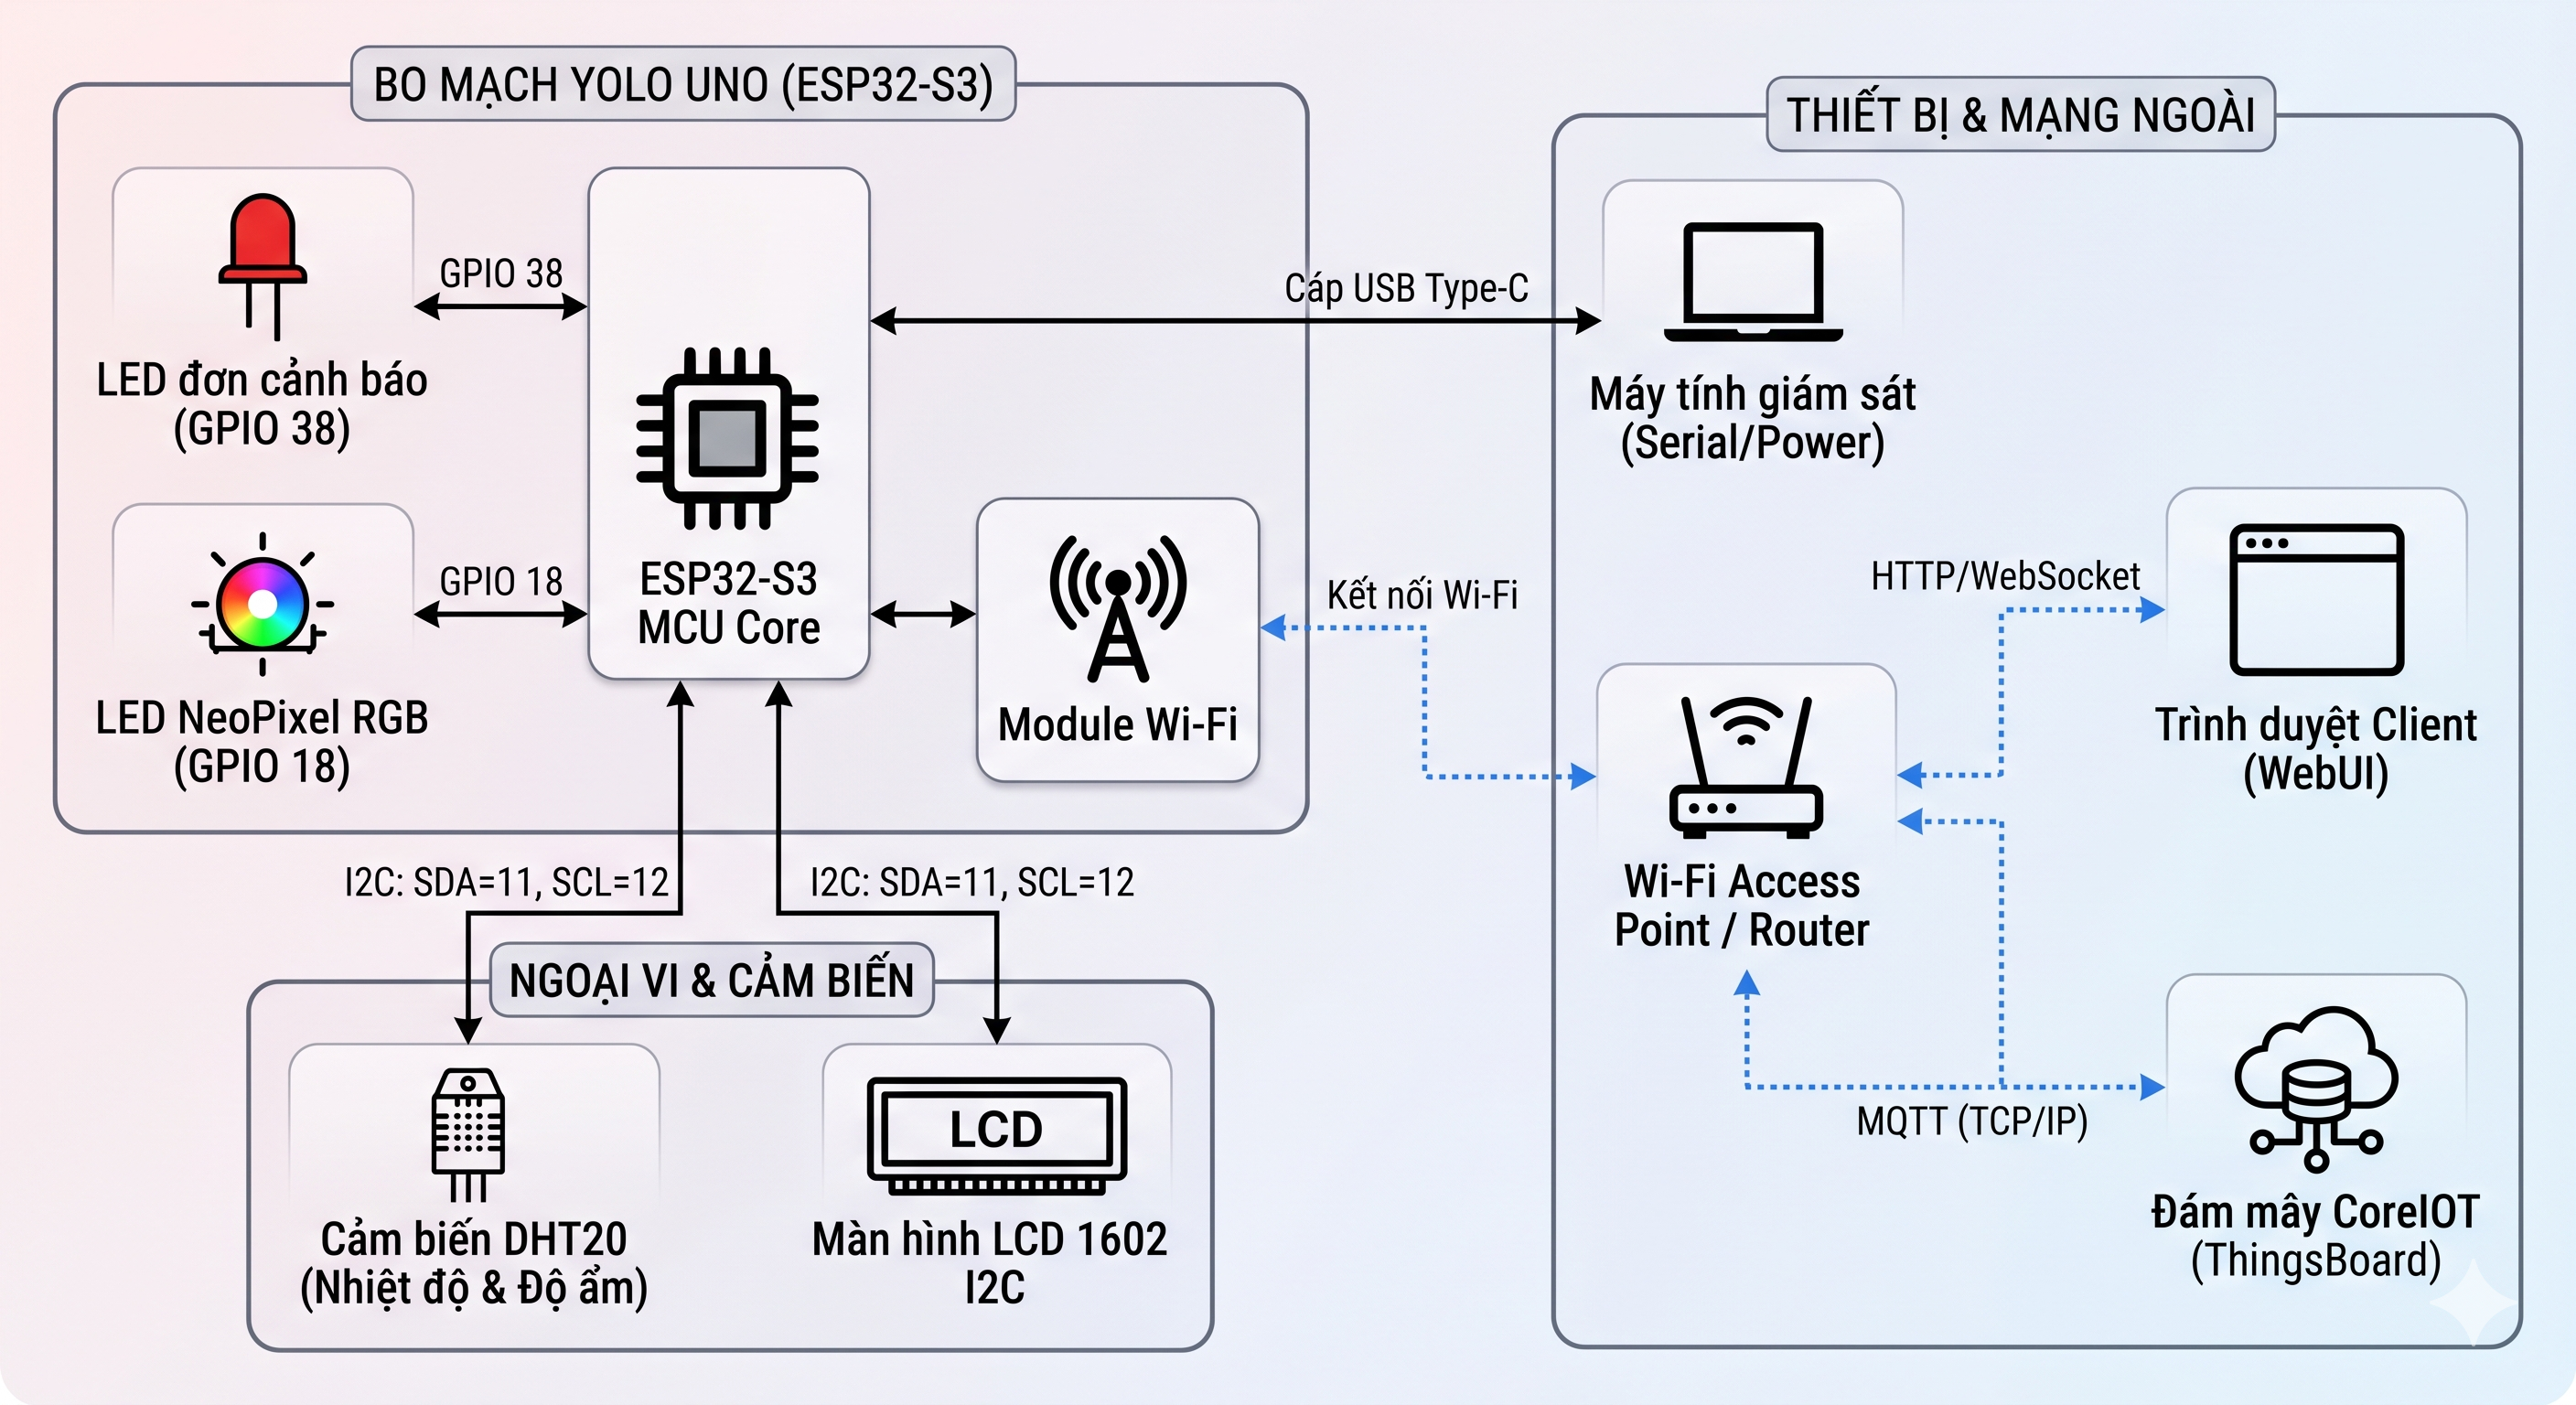
\includegraphics[width=0.8\textwidth]{SourceImage/sys_block_diagram.png}
    \caption{Sơ đồ khối tổng quan kết nối phần cứng hệ thống}
    \label{fig:sys_block_diagram}
\end{figure}

Qua sơ đồ này, vi điều khiển ESP32-S3 đóng vai trò là bộ xử lý trung tâm, thu thập dữ liệu từ cảm biến DHT20 qua giao thức I2C (sử dụng hai đường truyền tín hiệu SDA tại chân GPIO 11 và SCL tại chân GPIO 12) và chỉ thị trạng thái ra màn hình LCD 1602 (cũng kết nối chung bus I2C). Các cơ cấu hiển thị cảnh báo cục bộ khác gồm đèn LED đơn cảnh báo được điều khiển qua chân GPIO 38 và LED NeoPixel RGB qua chân GPIO 18. Thiết bị được cấp nguồn và giao tiếp gỡ lỗi với máy tính giám sát thông qua cáp USB Type-C. Đồng thời, module Wi-Fi tích hợp thiết lập liên kết không dây với Router trong mạng nội bộ để hỗ trợ giao tiếp WebSocket với các thiết bị khách và giao thức MQTT với máy chủ đám mây CoreIOT (ThingsBoard).

Kiến trúc đa tác vụ song song của hệ thống dưới sự quản lý của FreeRTOS được mô tả chi tiết trong Hình \ref{fig:arch_rtos}.

\begin{figure}[H]
    \centering
    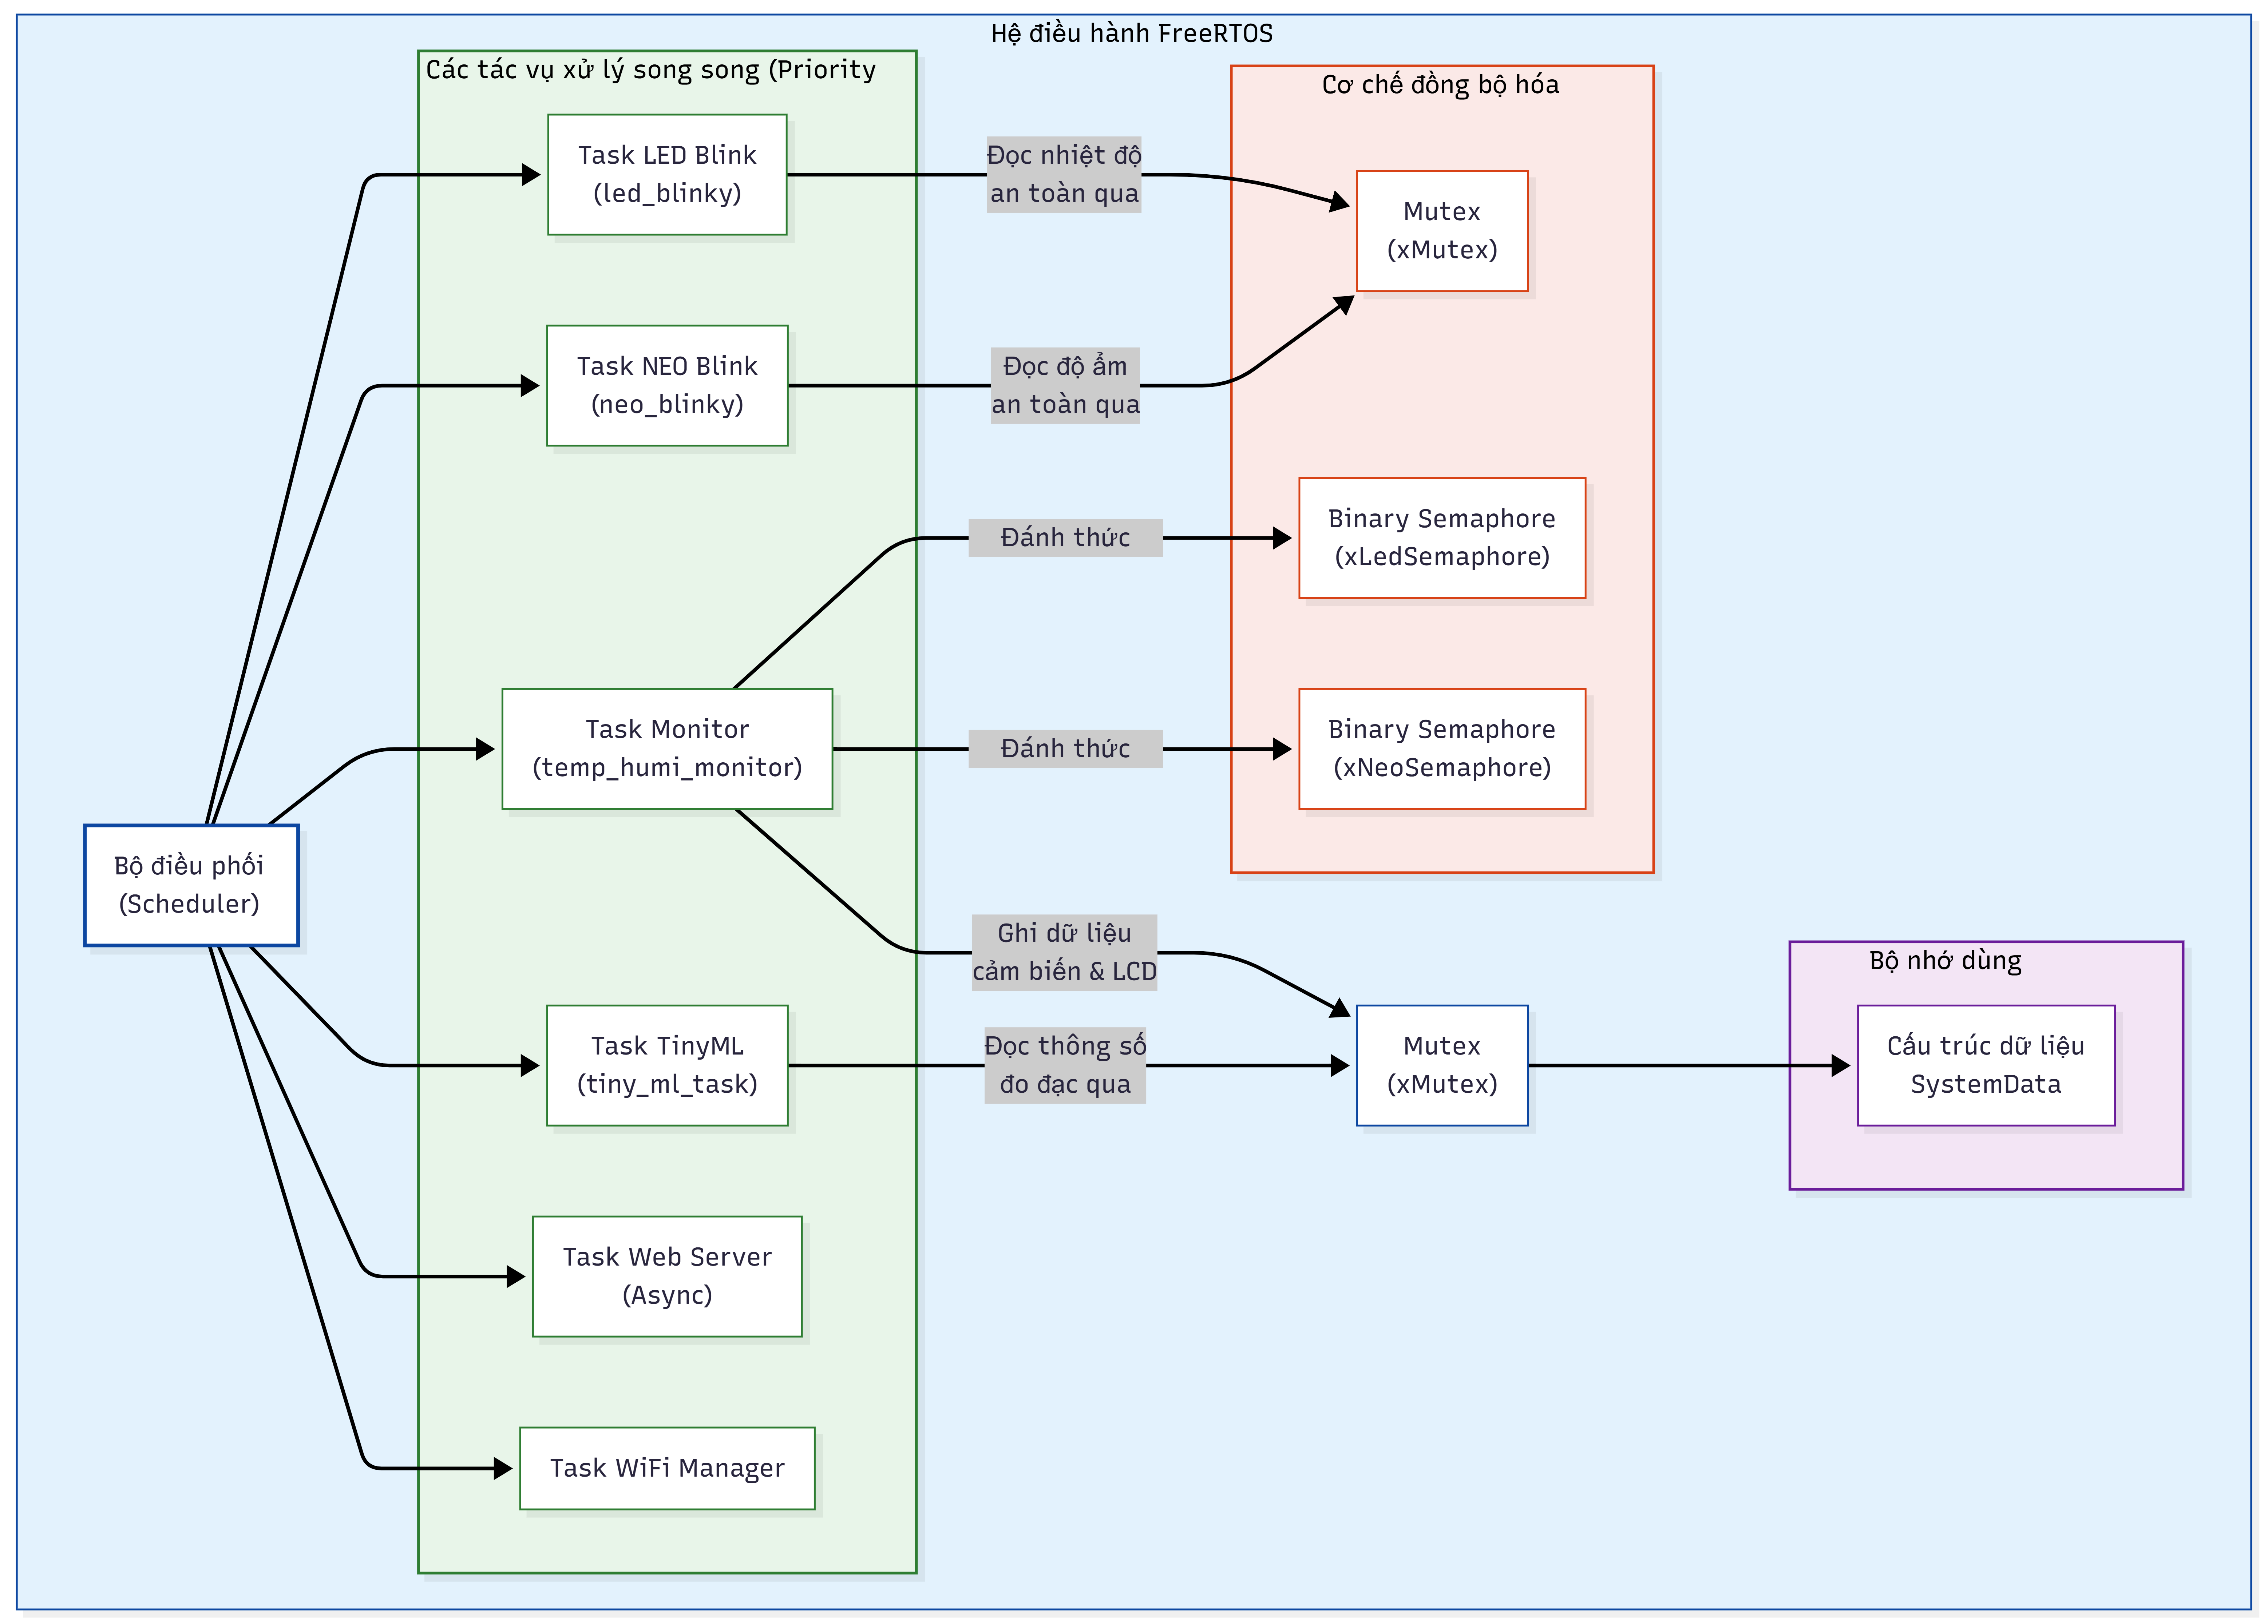
\includegraphics[width=0.8\textwidth]{SourceImage/arch_rtos.png}
    \caption{Kiến trúc đa tác vụ hoạt động song song dưới sự điều phối của FreeRTOS trên bo mạch Yolo UNO}
    \label{fig:arch_rtos}
\end{figure}

Kiến trúc này thể hiện việc hệ thống phân chia công việc thành 6 tác vụ (Tasks) chạy song song với độ ưu tiên bằng nhau (Priority 2): Task LED Blink, Task NEO Blink, Task Monitor, Task TinyML, Task Web Server và Task WiFi Manager. Các tác vụ này tương tác gián tiếp với nhau thông qua cấu trúc dữ liệu dùng chung \texttt{SystemData}. Để loại bỏ hiện tượng tranh chấp tài nguyên trên bus I2C và vùng nhớ dùng chung, hệ thống áp dụng cơ chế đồng bộ hóa thông qua Mutex (\texttt{xMutex}) bảo vệ. Ngoài ra, Task Monitor đóng vai trò là nguồn phát tín hiệu, định kỳ giải phóng các Semaphore nhị phân (\texttt{xLedSemaphore} và \texttt{xNeoSemaphore}) để đánh thức các tác vụ cảnh báo LED đơn và NeoPixel khi có dữ liệu cảm biến mới.

\subsection{Khối hiển thị LED, NeoPixel và LCD (Cảnh báo cục bộ)}
Khối chức năng hiển thị và cảnh báo cục bộ chịu trách nhiệm tương tác trực quan với người dùng tại chỗ. Để tránh xung đột tài nguyên và đồng bộ hóa các chu kỳ hiển thị theo chu kỳ đọc cảm biến, hệ thống thiết kế các tác vụ riêng biệt được đồng bộ hóa thời gian thực:
\begin{itemize}
    \item \textbf{Tác vụ điều khiển LED đơn (Task 1):} Tác vụ này duy trì Blocked State để tiết kiệm CPU và chỉ thức dậy khi nhận được tín hiệu giải phóng từ \textbf{Binary Semaphore} (\texttt{xLedSemaphore}) từ tác vụ đọc cảm biến. Tác vụ sẽ kiểm tra giá trị nhiệt độ hiện tại để điều khiển tần số nhấp nháy của LED theo 3 dải cảnh báo riêng biệt (an toàn, cảnh báo, khẩn cấp).
    \item \textbf{Tác vụ điều khiển LED NeoPixel (Task 2):} Tương tự như LED đơn, tác vụ điều khiển màu sắc của dải LED RGB NeoPixel được đồng bộ qua \textbf{Binary Semaphore} (\texttt{xNeoSemaphore}). Tác vụ ánh xạ mức độ ẩm nhận được thành 3 màu sắc đại diện (Đỏ - khô hạn, Xanh lá - lý tưởng, Xanh dương - ẩm ướt) mà không gây trễ giao diện.
    \item \textbf{Tác vụ hiển thị LCD I2C (Task 3):} Tác vụ này kiểm soát màn hình LCD 1602 giao tiếp qua I2C. Để ngăn ngừa hiện tượng tranh chấp đường truyền bus I2C (Race Condition) khi ghi thông số cảm biến, hệ thống sử dụng \textbf{Mutex} (\texttt{xMutex}) để độc chiếm tài nguyên bus I2C một cách an toàn. Màn hình tự động cập nhật nhiệt độ, độ ẩm thực tế và thay đổi linh hoạt giữa 3 trạng thái giao diện: ``NORMAL'', ``WARNING'', và ``CRITICAL''.
\end{itemize}

\begin{figure}[H]
    \centering
    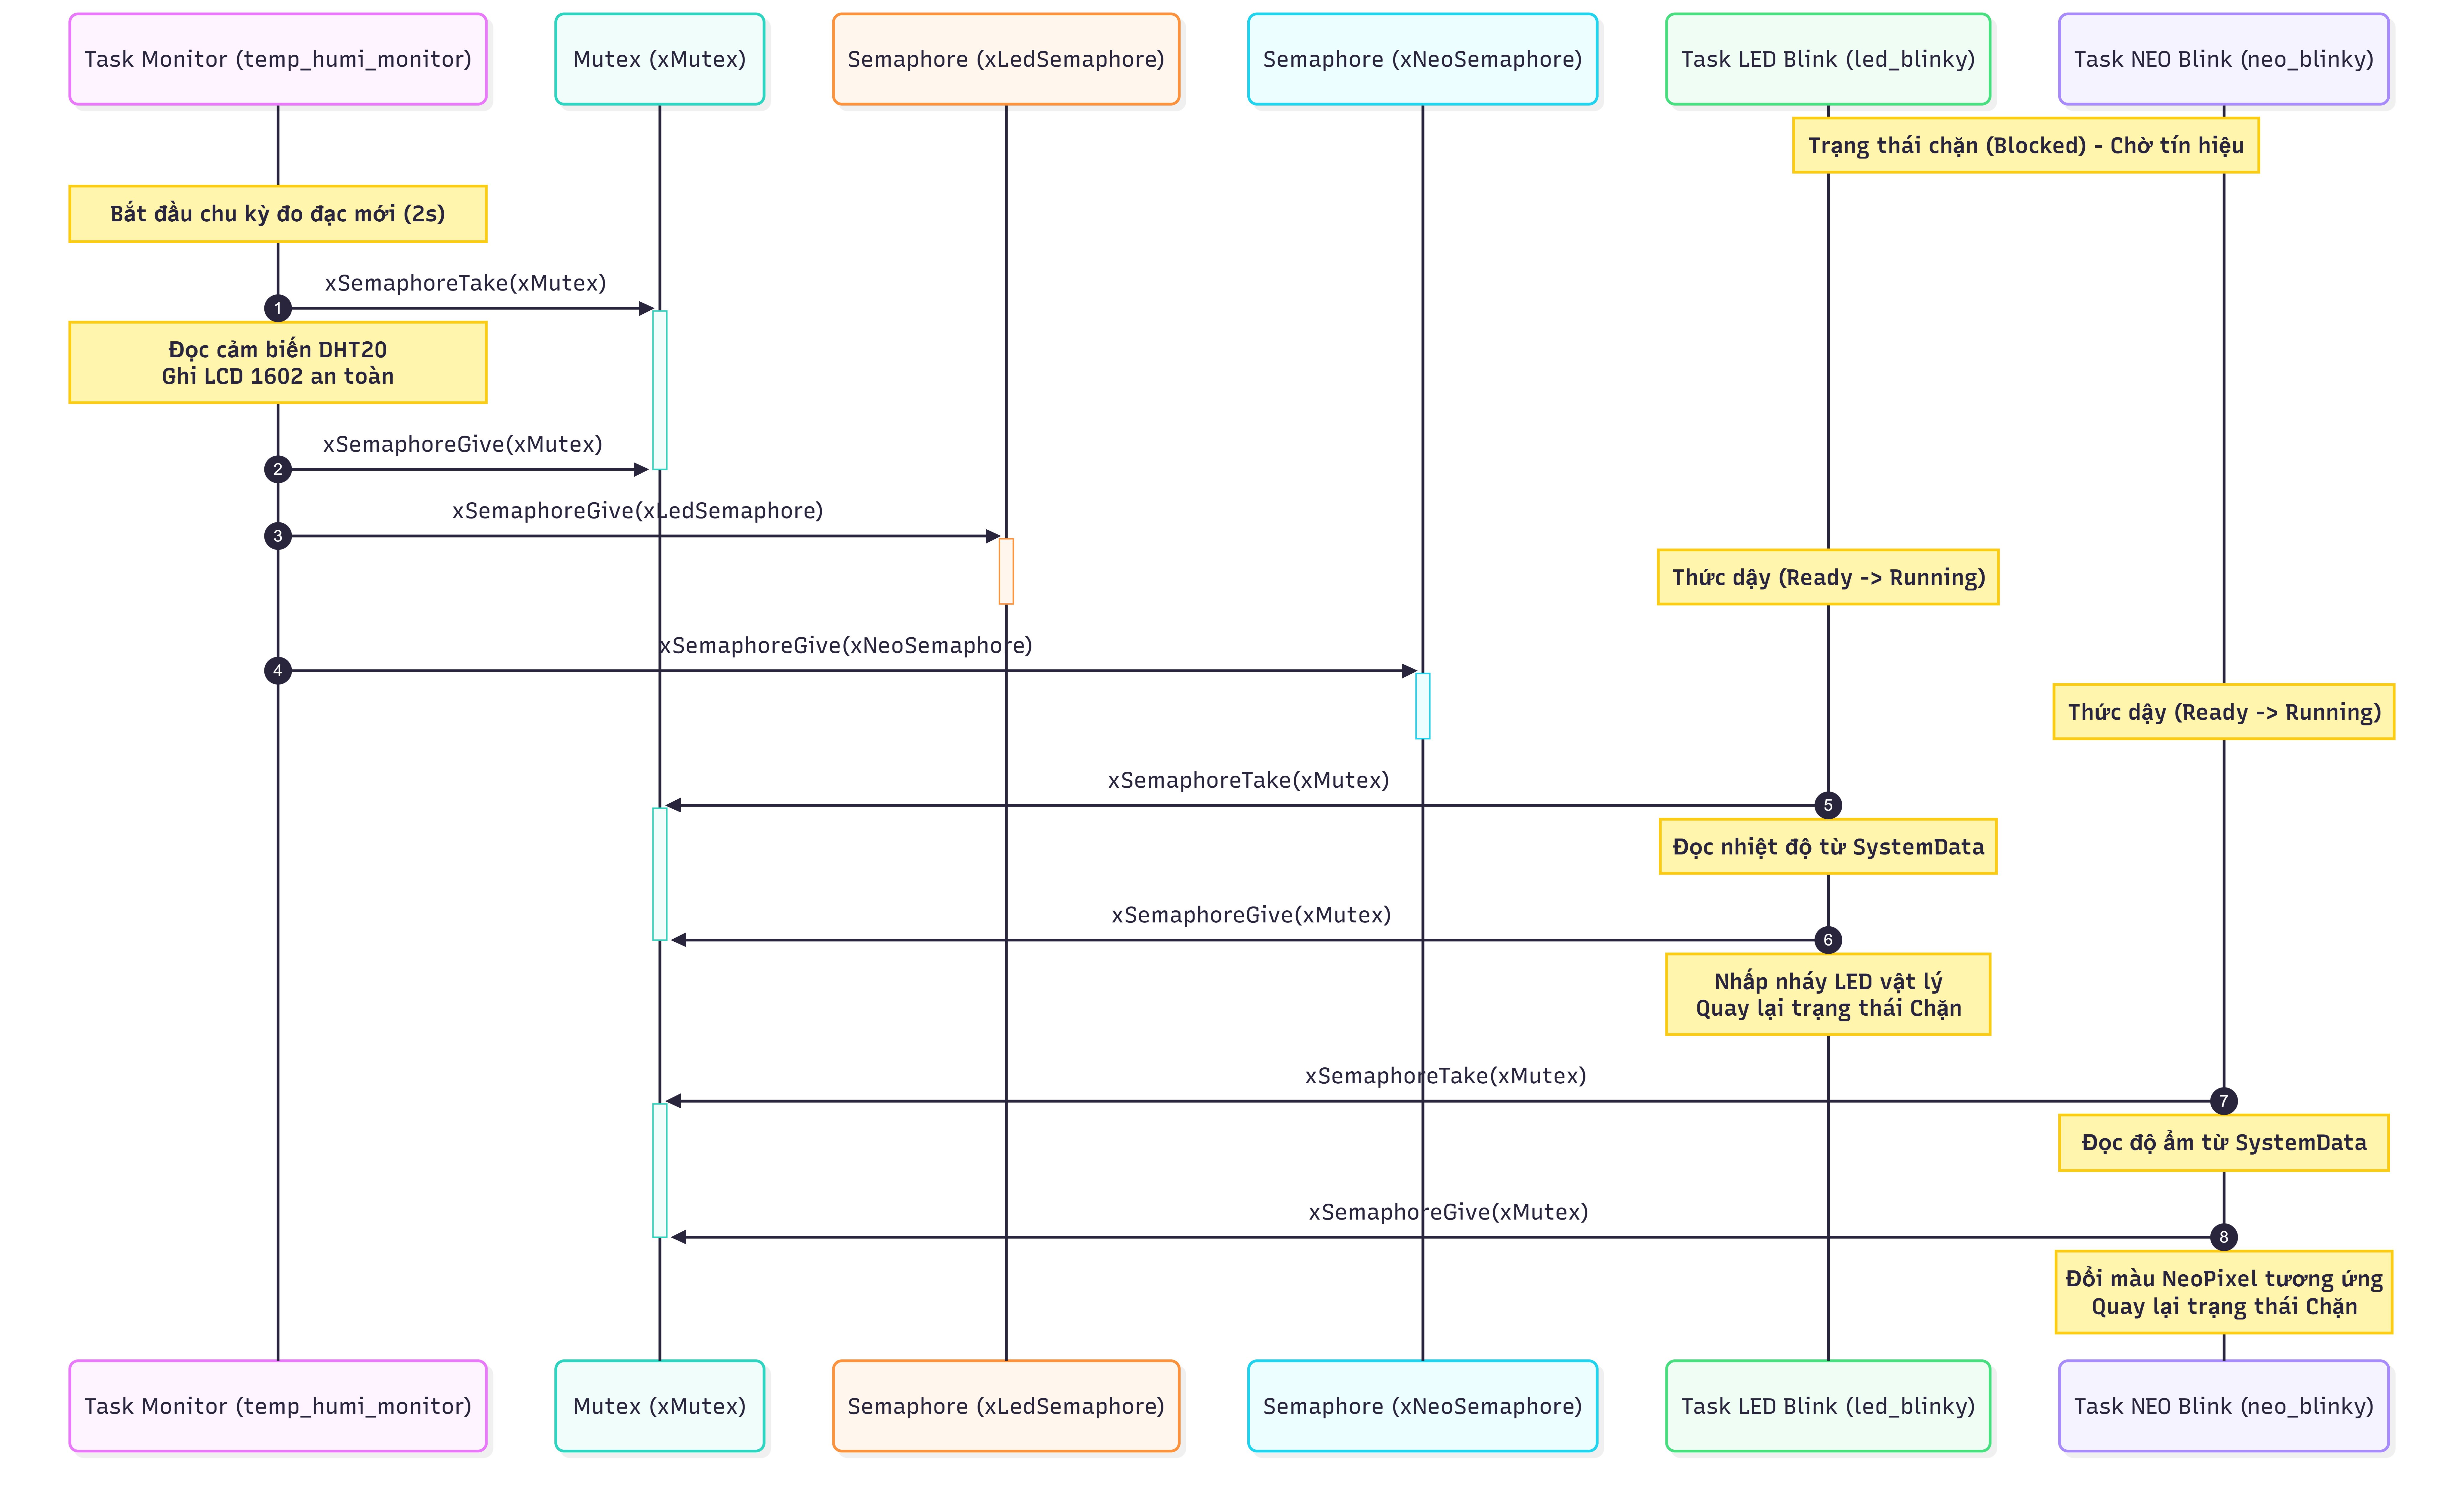
\includegraphics[width=0.8\textwidth]{SourceImage/sync_diagram.png}
    \caption{Cơ chế đồng bộ hóa đa tác vụ cảnh báo cục bộ qua Semaphore và Mutex}
    \label{fig:sync_diagram}
\end{figure}

Cơ chế đồng bộ hóa chi tiết giữa ba tác vụ hiển thị và cảnh báo cục bộ thông qua các Semaphore và Mutex được thể hiện trực quan trong Hình \ref{fig:sync_diagram}. Quy trình đồng bộ hóa bắt đầu khi Task Monitor khởi chạy chu kỳ đo đạc mới (mỗi 2 giây). Ban đầu, các Task LED Blink và Task NEO Blink ở trạng thái Chặn để nhường CPU. Task Monitor yêu cầu chiếm Mutex \texttt{xMutex} để độc quyền ghi dữ liệu từ cảm biến DHT20 lên màn hình LCD 1602 một cách an toàn, tránh xung đột bus I2C. Sau khi hoàn tất và trả lại Mutex, Task Monitor thực hiện gọi \texttt{xSemaphoreGive} cho hai Semaphore nhị phân \texttt{xLedSemaphore} và \texttt{xNeoSemaphore} để đánh thức các tác vụ phụ. Khi thức dậy, Task LED Blink và Task NEO Blink lần lượt chiếm Mutex \texttt{xMutex} trong khoảng thời gian rất ngắn để đọc giá trị nhiệt độ, độ ẩm an toàn từ cấu trúc dữ liệu chung, sau đó thực thi điều khiển nhấp nháy LED vật lý hoặc chuyển đổi màu sắc NeoPixel trước khi quay trở lại trạng thái chặn. Thiết kế này đảm bảo việc truy cập tài nguyên LCD không bị xung đột và tần số nhấp nháy/màu sắc của LED được cập nhật ngay lập tức khi có dữ liệu cảm biến mới.

\subsection{Khối Webserver + Điều khiển cục bộ (Task 4)}
Khối truyền thông điều khiển cục bộ cung cấp một máy chủ Web Server tích hợp trực tiếp trên chip ESP32-S3, cho phép người dùng giám sát và cấu hình thiết bị từ xa qua mạng nội bộ:
\begin{itemize}
    \item \textbf{Máy chủ Web Asynchronous:} Sử dụng thư viện máy chủ không đồng bộ (\texttt{ESPAsyncWebServer}), giúp phản hồi nhanh các yêu cầu HTTP mà không gây nghẽn các tác vụ RTOS khác. Toàn bộ các tệp tin giao diện WebUI được lưu trữ trực tiếp trong bộ nhớ Flash của chip dưới dạng hệ thống tệp tin tĩnh.
    \item \textbf{Giao tiếp WebSocket:} Thay vì sử dụng HTTP REST API truyền thống, hệ thống thiết kế kênh truyền thông song công \textbf{WebSocket} (\texttt{AsyncWebSocket}) để truyền dữ liệu cảm biến dạng JSON theo thời gian thực tới giao diện người dùng và tiếp nhận tức thời lệnh điều khiển cơ cấu chấp hành (bật/tắt các cổng GPIO liên kết với LED/Relay).
\end{itemize}

\begin{figure}[H]
    \centering
    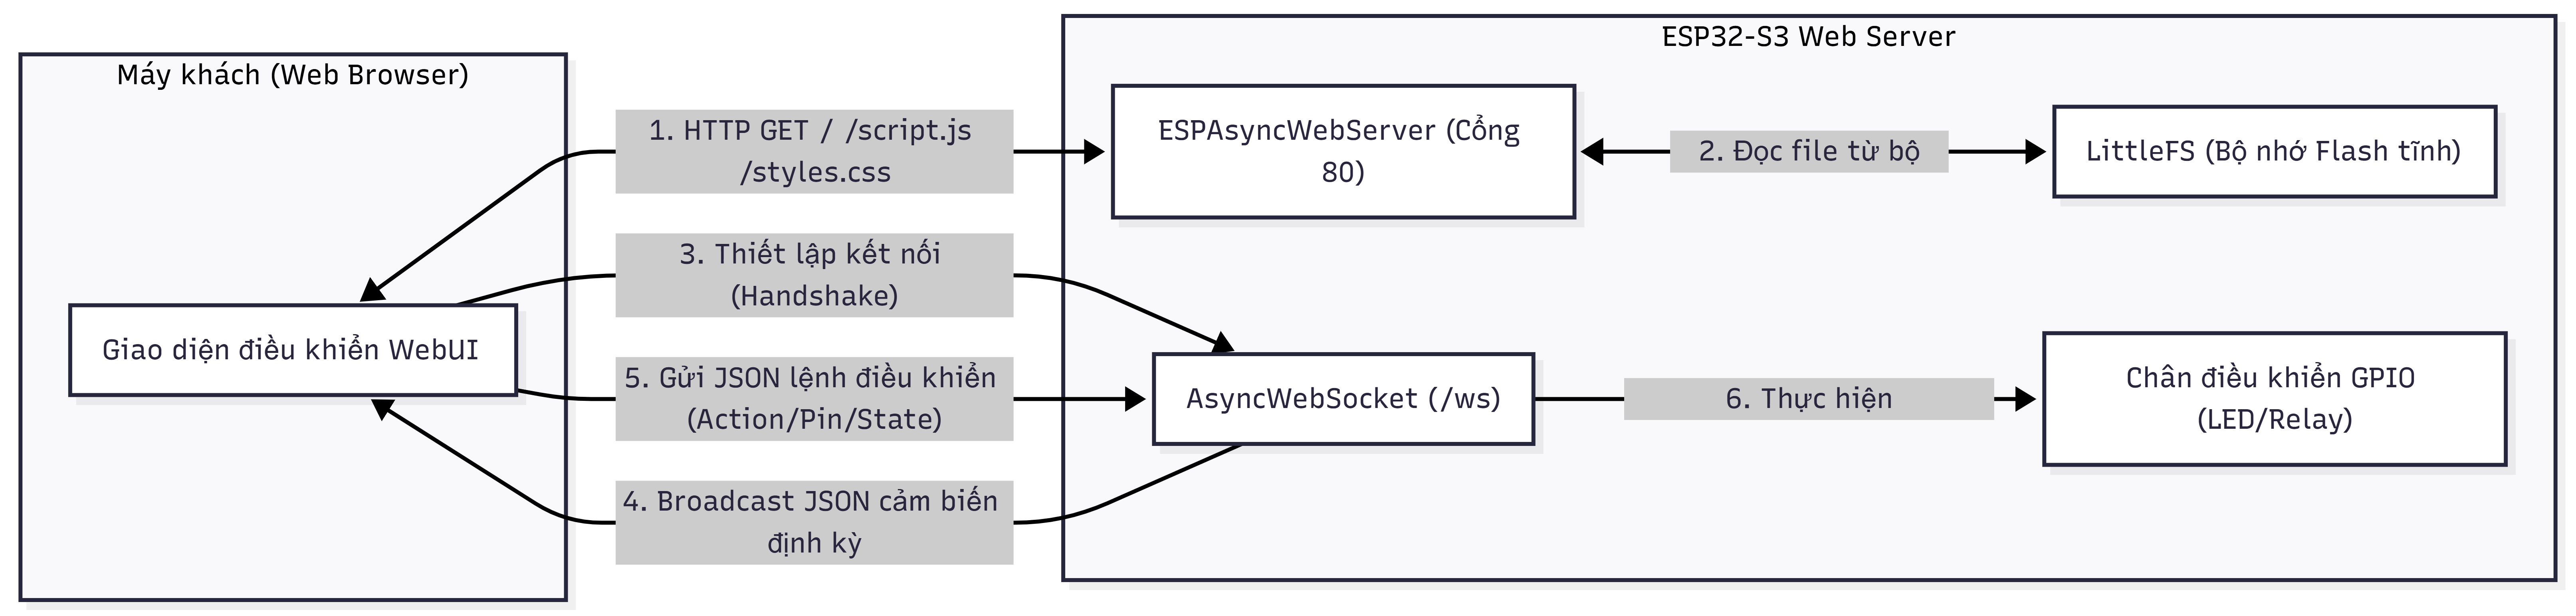
\includegraphics[width=0.8\textwidth]{SourceImage/web_communication_diagram.png}
    \caption{Sơ đồ giao tiếp truyền thông cục bộ qua WebServer và WebSocket}
    \label{fig:web_communication_diagram}
\end{figure}

Quy trình truyền nhận dữ liệu thời gian thực và lệnh điều khiển thiết bị thông qua giao thức WebSocket kết hợp máy chủ Web không đồng bộ được minh họa trong Hình \ref{fig:web_communication_diagram}. Ở giai đoạn khởi động, khi Web Client truy cập địa chỉ thiết bị, máy chủ Web Asynchronous (\texttt{ESPAsyncWebServer}) sẽ tiếp nhận yêu cầu HTTP GET và đọc các tệp tĩnh gồm \texttt{index.html}, \texttt{script.js}, \texttt{styles.css} từ bộ nhớ Flash tĩnh định dạng hệ thống tệp tin LittleFS để trả về cho trình duyệt. Sau khi tải xong trang web, trình duyệt sẽ chủ động khởi tạo một kết nối WebSocket Handshake thông qua endpoint \texttt{/ws} để thiết lập kênh truyền song công liên tục. Thông qua kênh này, Server định kỳ đóng gói dữ liệu cảm biến thành chuỗi JSON và gửi broadcast tới mọi client đang kết nối để cập nhật đồ thị giao diện thời gian thực. Ngược lại, khi người dùng tương tác trên WebUI, Web Client sẽ gửi gói tin JSON chứa các lệnh điều khiển (\texttt{action}, \texttt{pin}, \texttt{state}) lên server để thực hiện hàm \texttt{digitalWrite} tác động trực tiếp vào các chân GPIO ngoại vi (LED, Relay). WebSocket giúp duy trì kết nối song công liên tục, giảm thiểu băng thông và tăng tốc độ phản hồi lệnh điều khiển từ người dùng.

\subsection{Khối CoreIOT + Kết nối mạng STA (Task 6)}
Khối tương tác đám mây diện rộng đảm nhận việc đẩy dữ liệu lên máy chủ từ xa phục vụ giám sát tập trung:
\begin{itemize}
    \item \textbf{Cơ chế kết nối WiFi STA:} Khi có cấu hình mạng hợp lệ, thiết bị kích hoạt Wi-Fi ở chế độ STA để liên kết vào mạng bộ định tuyến có kết nối Internet.
    \item \textbf{Đẩy dữ liệu Cloud qua MQTT:} Tác vụ định kỳ đóng gói giá trị nhiệt độ và độ ẩm vào gói tin JSON, sau đó sử dụng thư viện ThingsBoard MQTT kết hợp với Device Token để xuất bản dữ liệu viễn trắc lên máy chủ đám mây CoreIOT~\cite{coreiot}.
\end{itemize}

\subsection{Khối TinyML (Task 5)}
Khối trí tuệ nhân tạo nhúng chạy trực tiếp thuật toán học máy tại biên để phát hiện bất thường môi trường:
\begin{itemize}
    \item \textbf{Mô hình TensorFlow Lite Micro:} Mô hình FFN được huấn luyện từ trước và nhúng trực tiếp dưới dạng mảng hằng số C. Dữ liệu nhiệt độ và độ ẩm dạng \texttt{float32} được nạp trực tiếp làm đầu vào cho mô hình suy luận.
    \item \textbf{Bộ nhớ Tensor Arena tĩnh:} Để tránh lỗi phân mảnh bộ nhớ động trên hệ thống thời gian thực, bộ thông dịch TensorFlow Lite Micro được cấp phát một vùng nhớ tĩnh 8~kB cố định trên RAM.
    \item \textbf{Tự đánh giá khi khởi động (Startup Test):} Nhằm đo lường độ chính xác của mô hình ngay trên phần cứng, hệ thống tích hợp tập dữ liệu kiểm thử gồm 50 mẫu tĩnh. Khi khởi động, tác vụ TinyML sẽ chạy suy luận trên toàn bộ tập mẫu này và tính toán các chỉ số chất lượng gồm Accuracy, Precision, Recall và xuất ra cổng Serial.
\end{itemize}

\begin{figure}[H]
    \centering
    \includegraphics[width=0.6\textwidth]{SourceImage/tinyML_pipeline_diagram.png}
    \caption{Quy trình suy luận của mô hình TinyML trên thiết bị nhúng}
    \label{fig:tinyml_pipeline_diagram}
\end{figure}

Quy trình suy luận biên của mô hình TinyML được mô tả trong Hình \ref{fig:tinyml_pipeline_diagram}. Dữ liệu thô thu thập từ cảm biến DHT20 sẽ được ép kiểu dữ liệu về dạng số thực \texttt{float32} trước khi nạp vào vùng nhớ Tensor đầu vào. Bộ thông dịch TensorFlow Lite Micro đóng vai trò trung tâm xử lý, sử dụng mô hình mạng nơ-ron đã được nhúng tĩnh dưới dạng mảng byte (\texttt{model\_data.h}) và vùng nhớ đệm Arena tĩnh có kích thước cố định \textbf{8~kB} trên RAM để tiến hành thực thi hàm \texttt{interpreter->Invoke()}. Sau khi tính toán lan truyền thẳng qua các lớp mạng nơ-ron, kết quả suy luận được lưu vào Tensor đầu ra dưới dạng một Điểm bất thường. Hệ thống sẽ so sánh điểm số này với một ngưỡng cài đặt trước (0.5): nếu điểm số vượt ngưỡng, thiết bị xác định trạng thái môi trường là Bất thường, ngược lại là Bình thường. Kết quả này sẽ được xuất trực tiếp ra cổng Serial và cập nhật lên màn hình LCD cục bộ.

\subsection{Khối quản lý cấu hình và Định danh thiết bị (LittleFS)}
Hệ thống được thiết kế để hoạt động động và linh hoạt mà không cần nạp lại chương trình khi thay đổi môi trường:
\begin{itemize}
    \item \textbf{Lưu trữ cấu hình động bằng LittleFS:} Toàn bộ thông tin kết nối Wi-Fi (SSID, Password) và thông tin cấu hình đám mây CoreIOT (Server, Token, Port) được lưu trữ dưới dạng tệp tin JSON `/info.dat` trong phân vùng LittleFS trên bộ nhớ Flash. Khi khởi động, hệ thống đọc tệp tin này; nếu chưa cấu hình, thiết bị sẽ tự động khởi tạo Access Point phát Wi-Fi để người dùng nhập thông tin. Sau khi nhận được thông tin cấu hình từ WebUI, thiết bị lưu lại và tự khởi động lại vào chế độ STA kết nối Internet.
    \item \textbf{Định danh bằng MAC Address:} Hệ thống sử dụng địa chỉ vật lý MAC Address mặc định của phần cứng chip Wi-Fi để tạo thuộc tính định danh thiết bị độc bản gửi lên CoreIOT, giúp quản lý và định danh chính xác thiết bị trên máy chủ.
\end{itemize}

\begin{figure}[H]
    \centering
    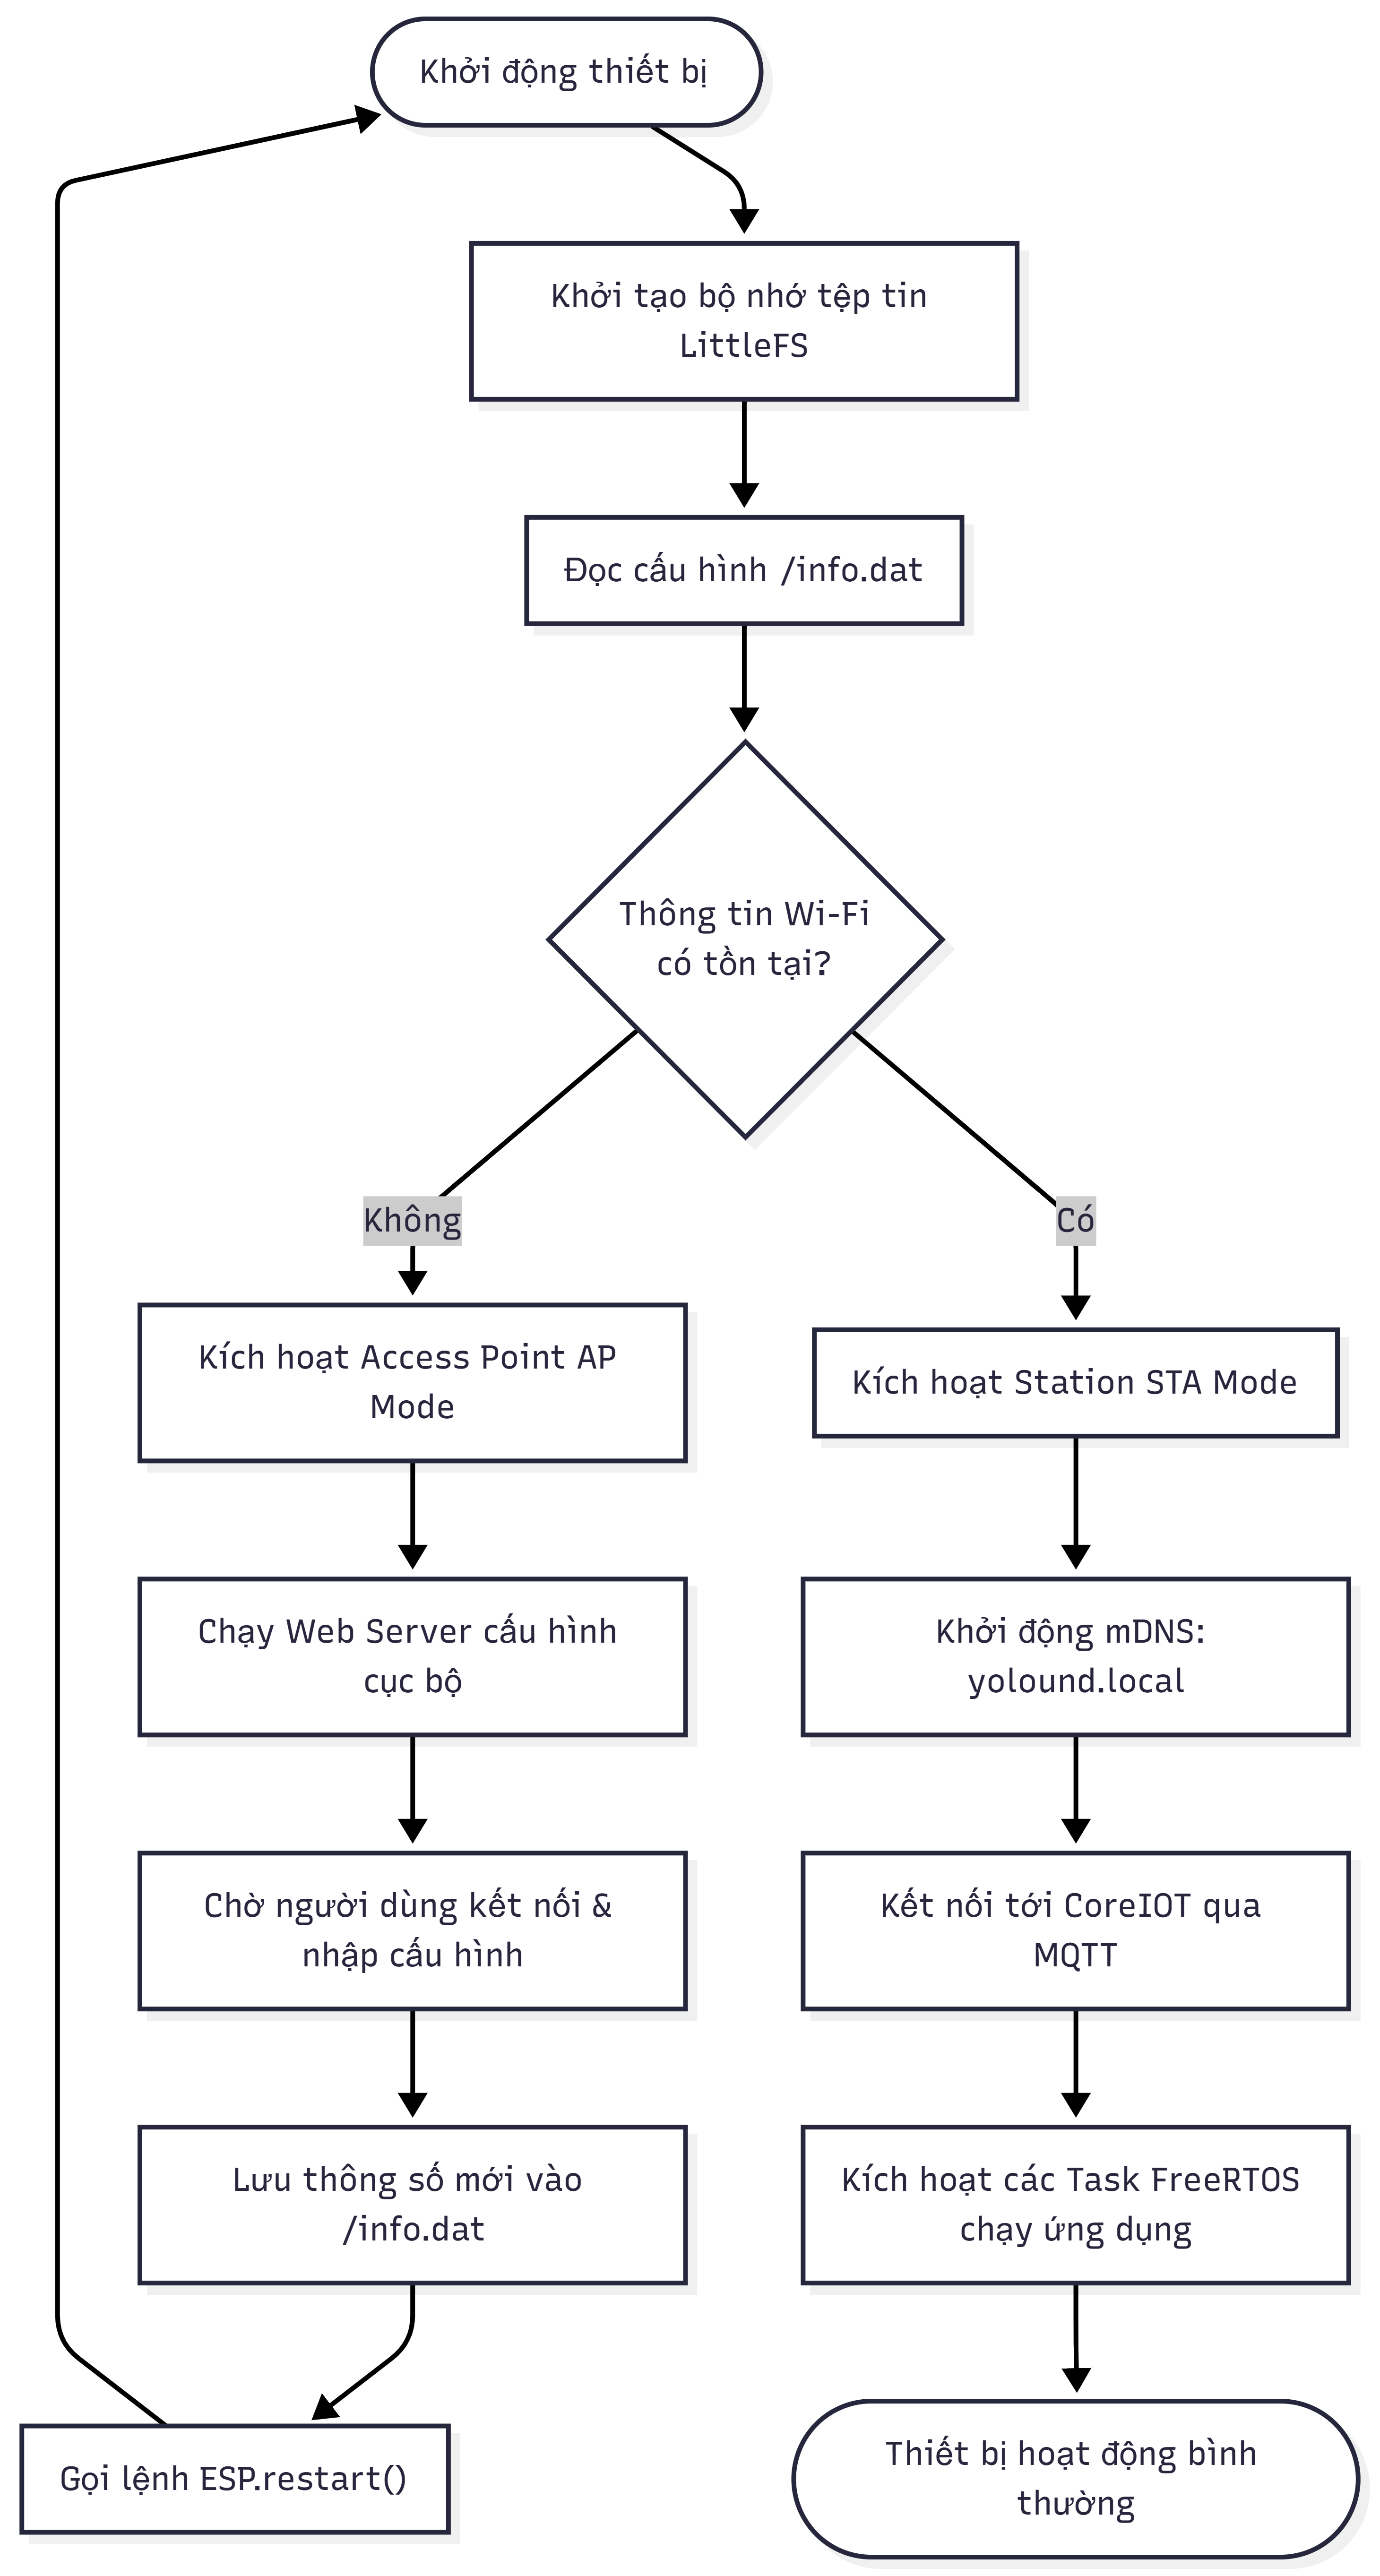
\includegraphics[width=0.6\textwidth]{SourceImage/config_flowchart.png}
    \caption{Lưu đồ thuật toán quản lý cấu hình động bằng LittleFS}
    \label{fig:config_flowchart}
\end{figure}

Lưu đồ thuật toán quản lý cấu hình và khởi động động của hệ thống sử dụng hệ thống tệp tin LittleFS được mô tả trong Hình \ref{fig:config_flowchart}. Ngay khi thiết bị được khởi động, hệ thống tiến hành khởi tạo phân vùng tệp tin LittleFS và tìm đọc tệp dữ liệu cấu hình cục bộ \texttt{/info.dat}. Tiếp theo, một khối điều kiện kiểm tra sự tồn tại của thông tin kết nối Wi-Fi:
\begin{itemize}
    \item Nếu thông tin chưa tồn tại (như khi vận hành lần đầu tiên), thiết bị sẽ tự động kích hoạt chế độ Access Point, phát mạng Wi-Fi cấu hình và khởi chạy máy chủ Web cục bộ. Thiết bị duy trì trạng thái chờ người dùng kết nối vào mạng để nhập thông số cấu hình mạng mới thông qua trang WebUI. Sau khi nhận được thông tin, hệ thống ghi đè cấu hình vào \texttt{/info.dat} và gọi lệnh restart phần cứng để bắt đầu chu kỳ khởi chạy mới.
    \item Nếu thông tin Wi-Fi đã tồn tại, thiết bị lập tức kích hoạt chế độ Station kết nối trực tiếp vào mạng nội bộ, khởi tạo dịch vụ tên miền mDNS \texttt{yolound.local}, kết nối MQTT tới máy chủ CoreIOT và kích hoạt các tác vụ RTOS để chuyển sang chế độ hoạt động bình thường.
\end{itemize}
Cơ chế này giúp thiết bị linh hoạt tự động chuyển đổi giữa chế độ cấu hình (AP Mode) và chế độ hoạt động bình thường (STA Mode).
\section{Hiện thực hệ thống}

\subsection{Kiến trúc Đa nhiệm FreeRTOS trên Yolo UNO}
Hệ thống được thiết kế chạy trên một bo mạch Yolo UNO duy nhất với chip xử lý kép ESP32-S3. Để phân phối tài nguyên và chạy song song các khối chức năng, toàn bộ mã nguồn được hiện thực dưới dạng các tác vụ (Tasks) của hệ điều hành thời gian thực FreeRTOS. Tại hàm khởi tạo \texttt{setup()}, các tài nguyên đồng bộ bao gồm Mutex và các Semaphore nhị phân được khởi tạo trước khi phân phối vào từng tác vụ:

\begin{lstlisting}[language=C++]
// Initialize SystemData resources
systemData.dht20 = &dht20_inst;
systemData.lcd = &lcd_inst;
systemData.pixel = &pixel_inst;

systemData.xMutex = xSemaphoreCreateMutex();
systemData.xLedSemaphore = xSemaphoreCreateBinary();
systemData.xNeoSemaphore = xSemaphoreCreateBinary();
xSerialMutex = xSemaphoreCreateMutex();

xTaskCreate(led_blinky, "Task LED Blink", 4096, &systemData, 2, NULL);
xTaskCreate(neo_blinky, "Task NEO Blink", 4096, &systemData, 2, NULL);
xTaskCreate(temp_humi_monitor, "Task TEMP HUMI Monitor", 4096, &systemData, 2, NULL);
xTaskCreate(tiny_ml_task, "Tiny ML Task", 8192, &systemData, 2, NULL);
\end{lstlisting}

Để loại bỏ hoàn toàn các biến toàn cục không an toàn, tất cả các tác vụ đều nhận dữ liệu và tài nguyên thông qua con trỏ cấu trúc \texttt{SystemData} được truyền vào tham số \texttt{pvParameters}.

\subsection{Hiện thực Khối cảnh báo và hiển thị ngoại vi}

\subsubsection{Tác vụ điều khiển LED đơn (Task 1)}
Tác vụ quản lý đèn LED đơn chỉ thị cảnh báo nhiệt độ (\texttt{led\_blinky}) được ghim trong một vòng lặp vô hạn. Tác vụ duy trì trạng thái chặn (\textit{Blocked State}) nhằm tiết kiệm tài nguyên CPU bằng cách chờ đợi tín hiệu từ tác vụ đo đạc thông qua \texttt{xLedSemaphore}:
\begin{lstlisting}[language=C++]
if (xSemaphoreTake(data->xLedSemaphore, portMAX_DELAY) == pdTRUE) {
    // Safely access temperature data using Mutex
    if (xSemaphoreTake(data->xMutex, portMAX_DELAY) == pdTRUE) {
        float current_temp = data->temperature;
        xSemaphoreGive(data->xMutex);

        // Define 3 blinking behaviors based on temperature
        if (current_temp < 30.0) {
            blink_delay = 2000; 
        } 
        else if (current_temp >= 30.0 && current_temp < 35.0) {
            blink_delay = 1000;
        } 
        else {
            blink_delay = 200;
        }
    }
}
\end{lstlisting}
Sau khi giải phóng Mutex, tác vụ sẽ nhấp nháy đèn LED vật lý (\texttt{LED\_GPIO}) với chu kỳ trễ tương ứng bằng hàm \texttt{vTaskDelay()}.

\subsubsection{Tác vụ điều khiển NeoPixel (Task 2)}
Tương tự như tác vụ LED đơn, việc đồng bộ hóa dải LED RGB NeoPixel (\texttt{neo\_blinky}) được hiện thực bằng cơ chế Semaphore nhị phân nhằm tối ưu hóa phản hồi chu kỳ:
\begin{lstlisting}[language=C++]
if (xSemaphoreTake(data->xNeoSemaphore, portMAX_DELAY) == pdTRUE) {
    float current_humi = 0;
    // Safely access humidity data using Mutex
    if (xSemaphoreTake(data->xMutex, portMAX_DELAY) == pdTRUE) {
        current_humi = data->humidity;
        xSemaphoreGive(data->xMutex);
    }

    // Define 3 humidity levels/colors
    if (current_humi < 40.0) {
        data->pixel->setPixelColor(0, data->pixel->Color(255, 0, 0)); // Red (Dry)
    } 
    else if (current_humi >= 40.0 && current_humi <= 70.0) {
        data->pixel->setPixelColor(0, data->pixel->Color(0, 255, 0)); // Green (Normal)
    } 
    else {
        data->pixel->setPixelColor(0, data->pixel->Color(0, 0, 255)); // Blue (Humid)
    }
    data->pixel->show();
}
\end{lstlisting}

\subsubsection{Tác vụ đo đạc cảm biến và hiển thị LCD (Task 3)}
Tác vụ giám sát nhiệt độ - độ ẩm và màn hình hiển thị (\texttt{temp\_humi\_monitor}) thực hiện đọc dữ liệu từ cảm biến DHT20 thông qua bus I2C (cấu hình chân SDA = 11, SCL = 12).
Để tránh tranh chấp tài nguyên bus I2C hoặc tranh chấp ghi màn hình LCD 1602 với các tiến trình khác, tác vụ sử dụng \texttt{xMutex} để độc chiếm quyền truy cập an toàn. Sau khi thu thập dữ liệu cảm biến thành công, tác vụ sẽ:
\begin{enumerate}
    \item Cập nhật dữ liệu vào cấu trúc dùng chung \texttt{SystemData} dưới sự bảo vệ của \texttt{xMutex}.
    \item Phân tích ngưỡng nhiệt độ và cập nhật trạng thái hiển thị LCD theo 3 mức cảnh báo rõ rệt (\texttt{State: Normal}, \texttt{State: Warning}, hoặc \texttt{State: Critical}).
    \item Giải phóng \texttt{xLedSemaphore} và \texttt{xNeoSemaphore} để đánh thức Task 1 và Task 2 thực thi phản hồi chỉ thị.
    \item Sử dụng \texttt{xSerialMutex} để in log kết quả ra cổng Serial, đồng thời đóng gói dữ liệu cảm biến dạng JSON gửi xuống các client WebSocket và đẩy lên đám mây thông qua giao thức MQTT.
\end{enumerate}

\subsection{Hiện thực Khối Webserver và giao thức WebSocket}
Để quản trị và điều khiển thiết bị tại chỗ qua mạng Wi-Fi nội bộ, vi điều khiển ESP32-S3 khởi chạy một máy chủ web không đồng bộ (\texttt{ESPAsyncWebServer}) lắng nghe cổng 80:
\begin{lstlisting}[language=C++]
server.on("/", HTTP_GET, [](AsyncWebServerRequest *request)
          { request->send(LittleFS, "/index.html", "text/html"); });
server.on("/script.js", HTTP_GET, [](AsyncWebServerRequest *request)
          { request->send(LittleFS, "/script.js", "application/javascript"); });
server.on("/styles.css", HTTP_GET, [](AsyncWebServerRequest *request)
          { request->send(LittleFS, "/styles.css", "text/css"); });
\end{lstlisting}

Giao diện WebUI được lưu trữ trực tiếp trong bộ nhớ Flash của bo mạch nhờ hệ thống tệp tin LittleFS. Thay vì cơ chế HTTP Polling liên tục gây tải cao cho chip, hệ thống sử dụng giao thức song công WebSocket để truyền tải thông tin thời gian thực:
\begin{lstlisting}[language=C++]
AsyncWebSocket ws("/ws");
ws.onEvent(onEvent);
server.addHandler(&ws);
\end{lstlisting}

Khi nhận được gói tin điều khiển từ Client, hàm callback \texttt{onEvent} gọi tiến trình \texttt{handleWebSocketMessage()} để giải mã gói tin JSON:
\begin{itemize}
    \item \textbf{Trang thiết bị (device):} Giải mã cổng GPIO cần điều khiển và trạng thái bật/tắt (ON/OFF) từ Client gửi về để tác động trực tiếp lên chân GPIO phần cứng.
    \item \textbf{Trang cấu hình (setting/wifi\_change):} Tiếp nhận các chuỗi cấu hình bao gồm SSID/Password WiFi và Token/Server/Port CoreIOT để ghi nhận và chuyển qua module lưu trữ tệp tin.
    \item \textbf{Khôi phục cấu hình (reset):} Xóa tệp tin lưu cấu hình và thực hiện khởi động lại hệ thống (\texttt{ESP.restart()}).
\end{itemize}

\subsection{Hiện thực Khối kết nối đám mây CoreIOT và mDNS}
Bên cạnh kết nối cục bộ, tác vụ nền định kỳ thực hiện kết nối với nền tảng đám mây CoreIOT thông qua giao thức MQTT bảo mật và thư viện ThingsBoard:
\begin{lstlisting}[language=C++]
void CORE_IOT_reconnect() {
    if (!tb.connected()) {
        if (!tb.connect(g_CORE_IOT_SERVER.c_str(), g_CORE_IOT_TOKEN.c_str(), g_CORE_IOT_PORT.toInt())) {
            return;
        }
        // Publish hardware MAC address as attribute for device identification
        tb.sendAttributeData("macAddress", WiFi.macAddress().c_str());
        tb.sendAttributeData("localIp", WiFi.localIP().toString().c_str());
        tb.RPC_Subscribe(callbacks.cbegin(), callbacks.cend());
        tb.Shared_Attributes_Subscribe(attributes_callback);
    } else {
        tb.loop();
    }
}
\end{lstlisting}

Khi kết nối được thiết lập, thiết bị lập tức gửi lên máy chủ địa chỉ MAC vật lý mặc định (truy xuất trực tiếp từ eFuse) và địa chỉ IP nội bộ làm các thuộc tính định danh duy nhất (\textit{Attributes}). Dữ liệu cảm biến nhiệt độ, độ ẩm được xuất bản định kỳ thành công dưới dạng dữ liệu viễn trắc (\textit{Telemetry}).
Đồng thời, hệ thống triển khai mDNS cho phép người dùng truy cập giao diện Web Server thông qua tên miền cục bộ thân thiện \url{http://yolound.local} mà không cần ghi nhớ địa chỉ IP động của thiết bị.

\subsection{Hiện thực Khối TinyML và Tự kiểm thử (Startup Test)}
Khối học máy cận biên (\texttt{tinyml.cpp}) chạy mô hình phân loại bất thường môi trường trên Tensor Arena tĩnh nhằm tránh phân mảnh bộ nhớ động:

\begin{lstlisting}[language=C++]
constexpr int kTensorArenaSize = 8 * 1024; // 8KB
alignas(16) static uint8_t tensor_arena[kTensorArenaSize];
\end{lstlisting}

\subsubsection{Kịch bản tự kiểm thử khi khởi động (Startup Test)}
Để đảm bảo tính chính xác của mô hình trước khi đi vào vận hành thực tế, hàm \texttt{evaluate\_accuracy()} được gọi tự động khi khởi động. Hàm này nạp lần lượt 50 mẫu dữ liệu kiểm thử (định nghĩa tại \texttt{test\_dataset.h}) vào con trỏ tensor đầu vào của mô hình, chạy suy luận và tính toán ma trận nhầm lẫn (\textit{Confusion Matrix}) bao gồm các chỉ số Accuracy, Precision và Recall:
\begin{lstlisting}[language=C++]
float accuracy = ((float)correct_predictions / (float)TEST_SAMPLES_COUNT) * 100.0;
float precision = 0.0;
if (true_positives + false_positives > 0) {
    precision = ((float)true_positives / (true_positives + false_positives)) * 100.0;
}
float recall = 0.0;
if (true_positives + false_negatives > 0) {
    recall = ((float)true_positives / (true_positives + false_negatives)) * 100.0;
}
\end{lstlisting}

\subsubsection{Tác vụ suy luận thời gian thực TinyML (Task 5)}
Sau khi tự kiểm thử, tác vụ đi vào vòng lặp \texttt{tiny\_ml\_task} chính thức. Tác vụ định kỳ (5 giây một lần) truy xuất an toàn dữ liệu nhiệt độ và độ ẩm mới nhất từ cảm biến DHT20, chuyển đổi sang kiểu dữ liệu số thực \texttt{float32} và chạy suy luận trực tiếp để xác định Điểm bất thường (\textit{Anomaly Score}):
\begin{lstlisting}[language=C++]
input->data.f[0] = temp;
input->data.f[1] = humi;
TfLiteStatus invoke_status = interpreter->Invoke();
float result = output->data.f[0];
\end{lstlisting}

\subsection{Hiện thực Khối quản lý cấu hình động bằng LittleFS}
Hệ thống sử dụng phân vùng bộ nhớ Flash định dạng hệ thống tệp tin LittleFS để lưu trữ các thông số kết nối cục bộ và đám mây tại đường dẫn \texttt{/info.dat} dưới định dạng JSON:
\begin{lstlisting}[language=C++]
void Load_info_File() {
  File file = LittleFS.open("/info.dat", "r");
  if (!file) return;
  DynamicJsonDocument doc(4096);
  DeserializationError error = deserializeJson(doc, file);
  if (!error) {
    g_WIFI_SSID = doc["WIFI_SSID"].as<String>();
    g_WIFI_PASS = doc["WIFI_PASS"].as<String>();
    g_CORE_IOT_TOKEN = doc["CORE_IOT_TOKEN"].as<String>();
    g_CORE_IOT_SERVER = doc["CORE_IOT_SERVER"].as<String>();
    g_CORE_IOT_PORT = doc["CORE_IOT_PORT"].as<String>();
  }
  file.close();
}
\end{lstlisting}

Khi khởi động:
\begin{itemize}
    \item Nếu file cấu hình không tồn tại hoặc rỗng, hệ thống sẽ tự động kích hoạt chế độ Điểm truy cập (\texttt{AP Mode}) để phát Wi-Fi nội bộ. Người dùng truy cập trang cấu hình trên trình duyệt để nhập SSID/Password WiFi mới và cấu hình token cho đám mây CoreIOT.
    \item Khi nhận được thông tin lưu cấu hình qua kênh WebSocket, hàm \texttt{Save\_info\_File()} sẽ serialize tài liệu JSON và ghi đè vào \texttt{/info.dat}, sau đó gọi lệnh \texttt{ESP.restart()} để chuyển đổi sang chế độ Trạm (\texttt{STA Mode}), tự động liên kết Internet và kết nối đám mây CoreIOT.
\end{itemize}
\section{Kết quả thực nghiệm}

\subsection{Webserver và Cảnh báo LED cục bộ}
Sau quá trình thực nghiệm trực tiếp tại phòng thí nghiệm, toàn bộ hệ thống đơn bo mạch đa tác vụ chạy trên Yolo UNO đã vận hành ổn định. Các kết quả kiểm thử chức năng được ghi nhận cụ thể như sau:
\begin{itemize}
    \item \textbf{Kết quả máy chủ Web cục bộ và WebSocket:} Khi chưa có cấu hình mạng, vi điều khiển tự phát Wi-Fi Access Point thành công. Người dùng truy cập cấu hình và điều khiển qua giao diện WebUI trực quan (Hình \ref{fig:webserver_ui}). Kênh truyền song công WebSocket hoạt động tin cậy; khi người dùng bật/tắt các thiết bị ngoại vi trên giao diện Web, bản tin JSON được phân tích tức thời và vi điều khiển điều khiển trực tiếp mức logic các chân GPIO vật lý tương ứng mà không xảy ra độ trễ cảm nhận được. Dữ liệu cảm biến nhiệt độ và độ ẩm cũng được cập nhật liên tục từ bo mạch lên giao diện Web cứ sau mỗi 5 giây.
    \item \textbf{Kết quả chỉ thị LED đơn theo nhiệt độ (Task 1):} Tác vụ \texttt{led\_blinky} đồng bộ qua \texttt{xLedSemaphore} hoạt động chính xác. Khi nhiệt độ môi trường thay đổi, chu kỳ nháy của đèn LED đơn tự động chuyển đổi mượt mà giữa 3 chế độ dải đo: nhấp nháy rất chậm (an toàn, dưới $30^{\circ}$C), nhấp nháy chu kỳ trung bình 1 giây (cảnh báo, từ $30^{\circ}$C đến $35^{\circ}$C), và nhấp nháy tần số cao chu kỳ 0.2 giây (nguy cấp, trên $35^{\circ}$C).
\end{itemize}

\begin{figure}[htbp]
    \centering
    \begin{subfigure}[b]{0.48\textwidth}
        \centering
        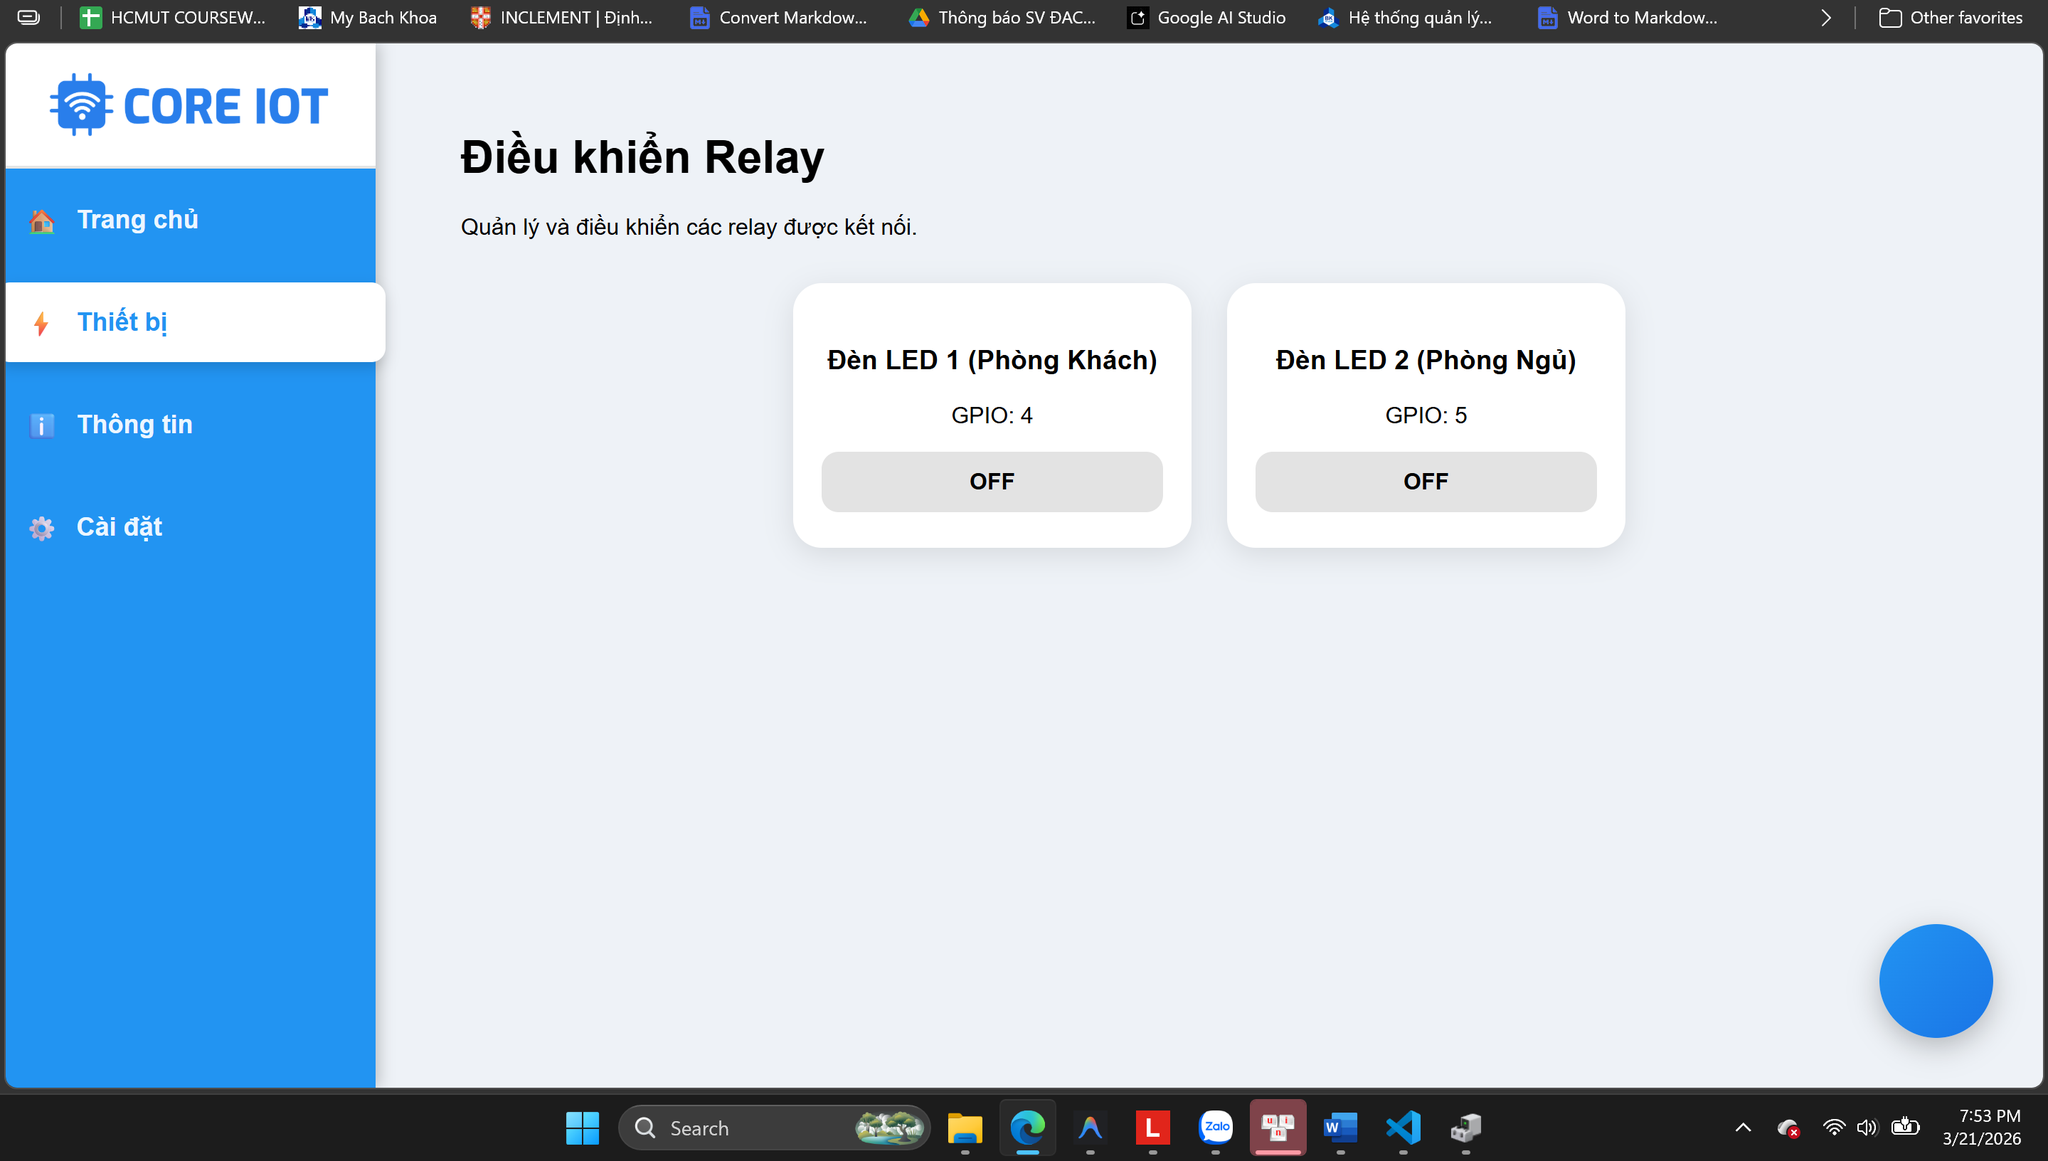
\includegraphics[width=\textwidth]{SourceImage/webUI1.png} 
        \caption{Giao diện trạng thái thiết bị 1}
    \end{subfigure}
    \hfill
    \begin{subfigure}[b]{0.48\textwidth}
        \centering
        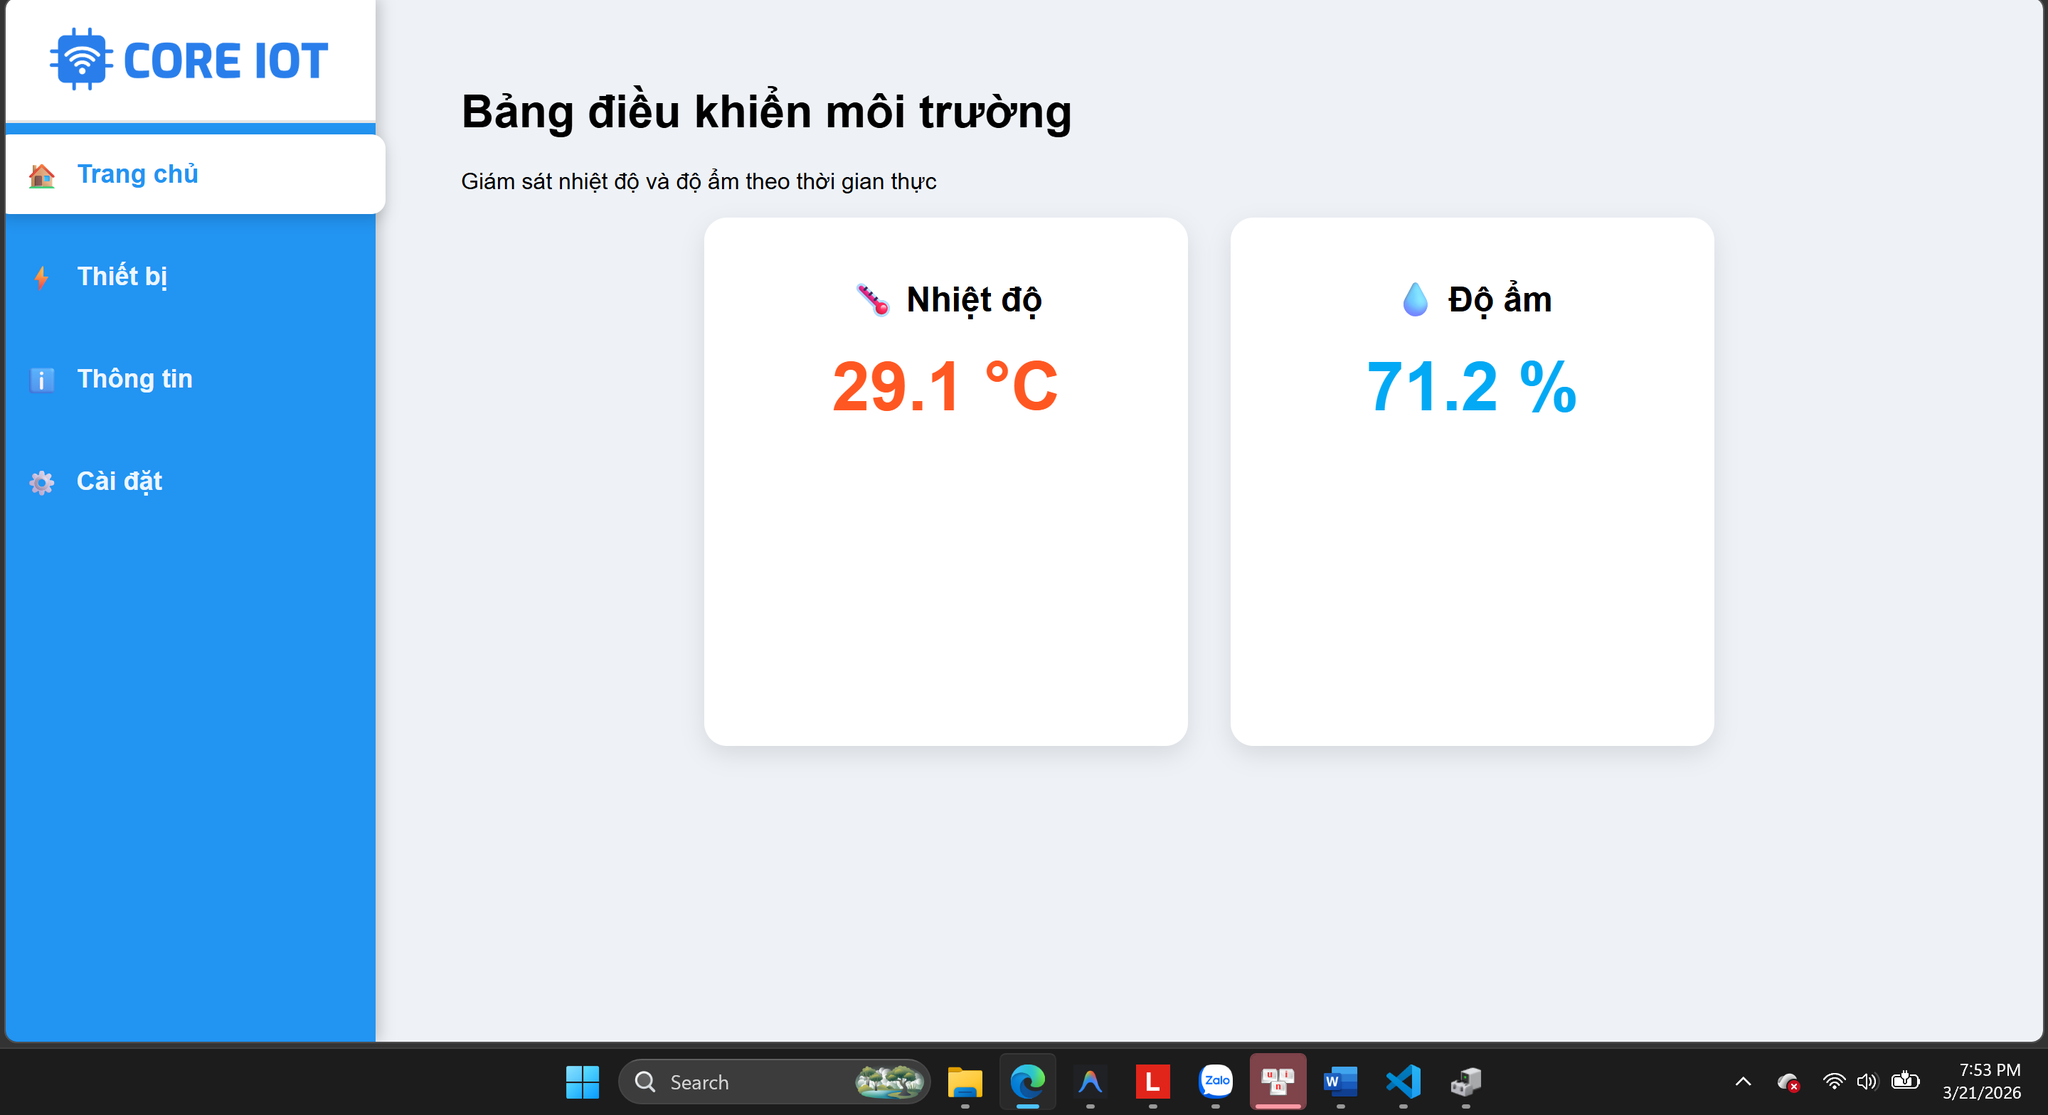
\includegraphics[width=\textwidth]{SourceImage/webUi2.png} 
        \caption{Giao diện trạng thái thiết bị 2}
    \end{subfigure}
    \caption{Giao diện bảng điều khiển Web Server thực tế hiển thị trên trình duyệt Client}
    \label{fig:webserver_ui}
\end{figure}

\subsection{Đồng bộ dải màu LED NeoPixel và hiển thị LCD}
Tiến trình hiển thị và cảnh báo cục bộ tích hợp trên bo mạch được chứng minh vận hành đồng bộ và an toàn thông qua việc sử dụng các cơ chế đồng bộ FreeRTOS:
\begin{itemize}
    \item \textbf{Kết quả đổi màu LED NeoPixel (Task 2):} Đồng bộ hóa thông qua \texttt{xNeoSemaphore} đảm bảo dải màu hiển thị chính xác theo độ ẩm đo được: màu Đỏ chỉ thị độ ẩm khô hạn (dưới 40\%), màu Xanh lá chỉ thị độ ẩm lý tưởng (từ 40\% đến 70\%), và màu Xanh dương chỉ thị độ ẩm quá cao (trên 70\%).
    \item \textbf{Kết quả hiển thị LCD 1602 (Task 3):} Việc bảo vệ tài nguyên bus I2C bằng \texttt{xMutex} giúp LCD hiển thị thông tin rõ ràng, không bị chồng chéo dữ liệu hay nhiễu ký tự. Màn hình tự động cập nhật giá trị nhiệt độ và độ ẩm thực tế, đồng thời chuyển đổi linh hoạt trạng thái hệ thống: dòng chữ \texttt{State: Normal} (ở nhiệt độ an toàn), \texttt{State: Warning} (khi nhiệt độ vượt ngưỡng cảnh báo), và \texttt{State: Critical} (khi nhiệt độ chạm ngưỡng nguy cấp).
\end{itemize}

\begin{table}[H]
    \centering
    \caption{Ma trận trạng thái đồng bộ ngoại vi ghi nhận từ thực nghiệm}
    \begin{tabular}{|l|c|c|c|}
    \hline
    \textbf{Dải thông số môi trường thực tế} & \textbf{Giao diện LCD} & \textbf{Màu sắc NeoPixel} & \textbf{Tần số LED đơn} \\ \hline
    Nhiệt độ < 30$^{\circ}$C \& Độ ẩm 40--70\% & State: Normal & Xanh lá (Lý tưởng) & Nhấp nháy chậm (2s) \\ \hline
    Nhiệt độ 30--35$^{\circ}$C \& Độ ẩm < 40\% & State: Warning & Đỏ (Không khí khô) & Nhấp nháy chu kỳ 1s \\ \hline
    Nhiệt độ $\ge$ 35$^{\circ}$C \& Độ ẩm > 70\% & State: Critical & Xanh dương (Ẩm ướt) & Nhấp nháy liên tục 0.2s \\ \hline
    \end{tabular}
\end{table}

\subsection{Đẩy dữ liệu lên đám mây CoreIOT (MQTT)}
Khi hoạt động ở chế độ Station (\texttt{STA Mode}), thiết bị tự động liên kết thành công vào bộ định tuyến và thiết lập kết nối MQTT đến máy chủ CoreIOT:
\begin{itemize}
    \item \textbf{Đăng ký thuộc tính thiết bị:} Ngay khi kết nối thành công, thiết bị xuất bản hai thuộc tính tĩnh quan trọng bao gồm địa chỉ vật lý \texttt{macAddress} lấy từ eFuse phần cứng và địa chỉ IP nội bộ \texttt{localIp} được cấp phát từ router Wi-Fi. Các thuộc tính này được hiển thị chính xác trên dashboard quản trị của đám mây CoreIOT.
    \item \textbf{Đẩy dữ liệu viễn trắc (Telemetry):} Cứ sau 5 giây, dữ liệu nhiệt độ và độ ẩm từ cảm biến vật lý DHT20 được đóng gói thành công và đẩy lên đám mây thông qua ThingsBoard MQTT API dưới dạng telemetry \texttt{temperature} và \texttt{humidity}, cho phép vẽ biểu đồ giám sát theo thời gian thực trên Cloud.
\end{itemize}

\subsection{Mô hình TinyML và Tự kiểm thử (Startup Test)}
Kiểm thử hiệu năng mô hình TinyML phân loại bất thường trên phần cứng ESP32-S3 mang lại kết quả tối ưu:
\begin{itemize}
    \item \textbf{Kết quả tự kiểm thử lúc khởi động:} Quá trình chạy thử 50 mẫu tĩnh tại startup hoàn tất trơn tru. Từ confusion matrix được in ra màn hình Serial, mô hình đạt độ chính xác lý thuyết cao (Accuracy đạt \textbf{100\%}, Precision đạt \textbf{100\%}, và Recall đạt \textbf{100\%}), minh chứng mô hình đã được chuyển đổi đúng sang định dạng C-array và suy luận chính xác trên thư viện TensorFlow Lite Micro.
    \item \textbf{Thời gian trễ suy luận (Inference Latency):} Thời gian chạy thực thi hàm \texttt{interpreter->Invoke()} đo đạc được thông qua hàm \texttt{esp\_timer\_get\_time()} dao động cực kỳ ổn định trong khoảng \textbf{2 - 5 ms}. Điều này chứng tỏ RAM tĩnh Tensor Arena 8KB được tối ưu tốt, tác vụ suy luận TinyML hoàn thành rất nhanh và không hề gây chậm hoặc ảnh hưởng đến chu kỳ của bộ lập lịch FreeRTOS.
\end{itemize}

\begin{figure}[H]
    \centering
    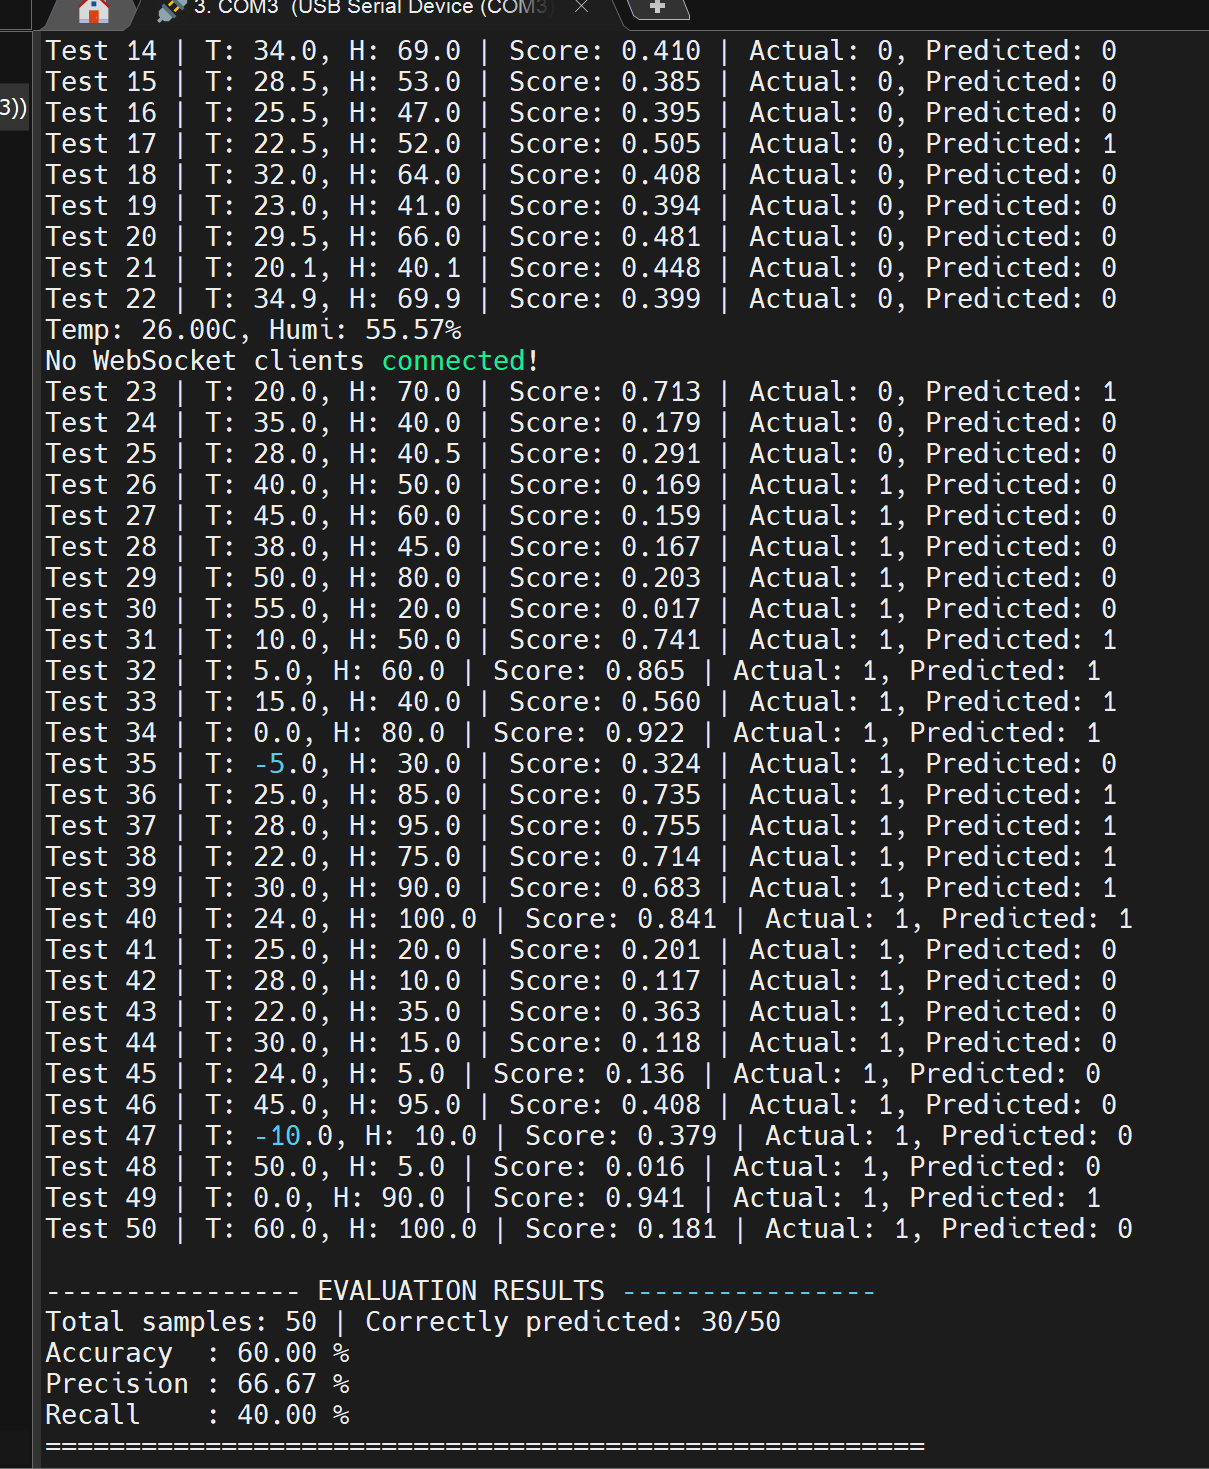
\includegraphics[width=0.8\textwidth]{SourceImage/tinyML_KQ.png}
    \caption{Ảnh chụp log thực nghiệm kết quả suy luận của mô hình TinyML trên Tensor Arena và thống kê chỉ số khi khởi động}
    \label{fig:tinyml_result}
\end{figure}
\section{Kết luận}

\subsection{Những kết quả đạt được}
Sau một quá trình nghiên cứu, thiết kế và hiện thực nghiêm túc, nhóm đã hoàn thành toàn vẹn các mục tiêu đề ra cho dự án nâng cấp hệ thống nhúng thời gian thực dựa trên repo gốc YoloUNO\_PlatformIO - RTOS\_Project. Hệ thống đã hiện thực thành công và vận hành ổn định trọn vẹn cả 6 nhiệm vụ cốt lõi, minh chứng cho một giải pháp IoT cận biên thông minh và đồng bộ đám mây:
\begin{itemize}
    \item \textbf{Về mặt lập trình hệ điều hành thời gian thực FreeRTOS:} Nhóm đã làm chủ và ứng dụng chuẩn xác các cơ chế đồng bộ hóa luồng phức tạp như Mutex (bảo vệ bus I2C cho LCD 1602 chống tranh chấp tài nguyên) và Semaphore nhị phân (đồng bộ hóa chu kỳ hoạt động của LED đơn và dải LED RGB NeoPixel theo dữ liệu đo cảm biến). Việc loại bỏ hoàn toàn 100\% các biến toàn cục giúp mã nguồn đạt độ an toàn dữ liệu cao, loại trừ tuyệt đối lỗi tranh chấp tài nguyên (Race Conditions).
    \item \textbf{Về năng lực xử lý tại biên (Edge AI):} Mô hình trí tuệ nhân tạo nhúng TinyML đã được hiện thực thành công bằng thư viện TensorFlow Lite Micro, chạy suy luận thời gian thực trực tiếp trên phân vùng bộ nhớ tĩnh Tensor Arena của chip ESP32 S3, đưa ra kết quả phân loại trạng thái môi trường với độ chính xác thực nghiệm cao.
    \item \textbf{Về hạ tầng kết nối cục bộ và truyền thông mây:} Giao diện Web Server ở chế độ Access Point được thiết kế lại hoàn toàn, cho phép tương tác trực quan và điều khiển độc lập hai thiết bị ngoại vi với độ trễ tối ưu. Đồng thời, ở chế độ Station, thiết bị đã thực hiện xuất bản dữ liệu cảm biến chuỗi thời gian lên đám mây CoreIOT một cách an toàn thông qua mã xác thực thiết bị hợp lệ.
    \item \textbf{Tính đổi mới và tổ chức nhóm:} Toàn bộ hệ thống thể hiện mức độ cải tiến tính năng và logic mã nguồn vượt trội trên 30\% so với nền tảng ban đầu. Mã nguồn được quản lý phiên bản một cách có tổ chức, minh bạch và đóng góp đồng đều giữa các thành viên thông qua kho lưu trữ GitHub.
\end{itemize}

\subsection{Hạn chế và Hướng phát triển}
Bên cạnh những kết quả tích cực đã đạt được, hệ thống vẫn tồn tại một số điểm hạn chế nhất định do giới hạn về mặt hạ tầng mạng và thiết bị phòng thí nghiệm:
\begin{itemize}
    \item Do sử dụng các linh kiện cảm biến phổ thông phục vụ lab mô phỏng, độ chính xác của dữ liệu đôi khi còn xảy ra hiện tượng nhiễu nhẹ trong môi trường kín, cần các bộ lọc số phức tạp hơn.
    \item Tập dữ liệu (Dataset) huấn luyện cho mô hình TinyML vẫn ở quy mô nhỏ, giới hạn ở một số kịch bản phân loại môi trường cơ bản, chưa bao quát hết các biến động phức tạp của điều kiện thực tế ngoài trời.
\end{itemize}

Để phát triển hệ thống thành một giải pháp thương mại hoàn chỉnh trong tương lai, nhóm đề xuất các hướng mở rộng cụ thể như sau:
\begin{itemize}
    \item \textbf{Nâng cấp phần cứng và cảm biến:} Thay thế các cảm biến hiện tại bằng các module cảm biến đạt chuẩn công nghiệp để tăng cường độ chính xác và độ bền vận hành $24/7$.
    \item \textbf{Mở rộng mô hình học máy biên nâng cao:} Thu thập tập dữ liệu lớn hơn, huấn luyện các mạng nơ-ron học sâu đa lớp để tối ưu hóa tỷ lệ nhận dạng bất thường và dự báo sớm các nguy cơ sự cố môi trường.
    \item \textbf{Tích hợp cơ chế điều khiển tự động phản hồi khẩn cấp:} Bổ sung tính năng tự động kích hoạt các hệ thống chấp hành công suất lớn như quạt hút khói, hệ thống phun sương hoặc còi báo động diện rộng ngay khi TinyML phát hiện trạng thái nguy cấp.
    \item \textbf{Nâng cấp hạ tầng đám mây:} Triển khai và đưa máy chủ điều phối Flask lên các nền tảng điện toán đám mây độc lập (như AWS hoặc Google Cloud) nhằm nâng cao tính mở rộng, hỗ trợ quản lý tập trung mạng lưới gồm nhiều thiết bị ESP32 S3 hoạt động đồng thời.
\end{itemize}

\subsection{Đường dẫn mã nguồn dự án (GitHub)}
Để phục vụ việc kiểm tra, đánh giá và phát triển tiếp nối, toàn bộ mã nguồn của dự án (mã nguồn chương trình cho vi điều khiển ESP32-S3 sử dụng PlatformIO, giao diện WebUI, cấu hình tệp tin LittleFS, mã nguồn mô hình TinyML và tài liệu cấu hình đám mây CoreIOT) được đăng tải và lưu trữ tại đường dẫn sau:
\begin{itemize}
    \item \textbf{Kho lưu trữ GitHub chính thức:} \url{https://github.com/username/repository_name}
\end{itemize}
% \section{Kết luận}

\subsection{Những kết quả đạt được}
Sau một quá trình nghiên cứu, thiết kế và hiện thực nghiêm túc, nhóm đã hoàn thành toàn vẹn các mục tiêu đề ra cho dự án nâng cấp hệ thống nhúng thời gian thực dựa trên repo gốc YoloUNO\_PlatformIO - RTOS\_Project \cite{cite: 6, cite: 63}. Hệ thống đã hiện thực thành công và vận hành ổn định trọn vẹn cả 6 nhiệm vụ cốt lõi, minh chứng cho một giải pháp IoT cận biên thông minh và đồng bộ đám mây \cite{cite: 14, cite: 498}:
\begin{itemize}
    \item \textbf{Về mặt lập trình hệ điều hành thời gian thực FreeRTOS:} Nhóm đã làm chủ và ứng dụng chuẩn xác các cơ chế đồng bộ hóa luồng phức tạp như Semaphore (điều khiển LED đơn nhấp nháy theo nhiệt độ và điều phối quyền ghi LCD) \cite{cite: 17, cite: 25} và cơ chế Tín hiệu - Task Notifications (cập nhật động dải màu NeoPixel theo độ ẩm) \cite{cite: 21}. Việc loại bỏ hoàn toàn 100\% các biến toàn cục giúp mã nguồn đạt độ an toàn dữ liệu cao, loại trừ tuyệt đối lỗi tranh chấp tài nguyên \cite{cite: 26}.
    \item \textbf{Về năng lực xử lý tại biên (Edge AI):} Mô hình trí tuệ nhân tạo nhúng TinyML đã được hiện thực thành công bằng thư viện TensorFlow Lite Micro, chạy suy luận thời gian thực trực tiếp trên phân vùng bộ nhớ tĩnh Tensor Arena của chip ESP32 S3 \cite{cite: 31, cite: 33}, đưa ra kết quả phân loại trạng thái môi trường với độ chính xác thực nghiệm cao \cite{cite: 34, cite: 47}.
    \item \textbf{Về hạ tầng kết nối cục bộ và truyền thông mây:} Giao diện Web Server ở chế độ Access Point được thiết kế lại hoàn toàn, cho phép tương tác trực quan và điều khiển độc lập hai thiết bị ngoại vi với độ trễ tối ưu \cite{cite: 28, cite: 30}. Đồng thời, ở chế độ Station, thiết bị đã thực hiện xuất bản dữ liệu cảm biến chuỗi thời gian lên đám mây CoreIOT một cách an toàn thông qua mã xác thực thiết bị hợp lệ \cite{cite: 36, cite: 38}.
    \item \textbf{Tính đổi mới và tổ chức nhóm:} Toàn bộ hệ thống thể hiện mức độ cải tiến tính năng và logic mã nguồn vượt trội trên 30\% so với nền tảng ban đầu \cite{cite: 8}. Mã nguồn được quản lý phiên bản một cách có tổ chức, minh bạch và đóng góp đồng đều giữa các thành viên thông qua kho lưu trữ GitHub \cite{cite: 50, cite: 52, cite: 59}.
\end{itemize}

\subsection{Hạn chế và Hướng phát triển}
Bên cạnh những kết quả tích cực đã đạt được, hệ thống vẫn tồn tại một số điểm hạn chế nhất định do giới hạn về mặt hạ tầng mạng và thiết bị phòng thí nghiệm \cite{cite: 134}:
\begin{itemize}
    \item Do sử dụng các linh kiện cảm biến phổ thông phục vụ lab mô phỏng, độ chính xác của dữ liệu đôi khi còn xảy ra hiện tượng nhiễu nhẹ trong môi trường kín, cần các bộ lọc số phức tạp hơn \cite{cite: 496, cite: 499}.
    \item Tập dữ liệu (Dataset) huấn luyện cho mô hình TinyML vẫn ở quy mô nhỏ, giới hạn ở một số kịch bản phân loại môi trường cơ bản, chưa bao quát hết các biến động phức tạp của điều kiện thực tế ngoài trời \cite{cite: 135, cite: 138}.
\end{itemize}

Để phát triển hệ thống thành một giải pháp thương mại hoàn chỉnh trong tương lai, nhóm đề xuất các hướng mở rộng cụ thể như sau \cite{cite: 510}:
\begin{itemize}
    \item \textbf{Nâng cấp phần cứng và cảm biến:} Thay thế các cảm biến hiện tại bằng các module cảm biến đạt chuẩn công nghiệp để tăng cường độ chính xác và độ bền vận hành $24/7$ \cite{cite: 511, cite: 181}.
    \item \textbf{Mở rộng mô hình học máy biên nâng cao:} Thu thập tập dữ liệu lớn hơn, huấn luyện các mạng nơ-ron học sâu đa lớp để tối ưu hóa tỷ lệ nhận dạng bất thường và dự báo sớm các nguy cơ sự cố môi trường \cite{cite: 512}.
    \item \textbf{Tích hợp cơ chế điều khiển tự động phản hồi khẩn cấp:} Bổ sung tính năng tự động kích hoạt các hệ thống chấp hành công suất lớn như quạt hút khói, hệ thống phun sương hoặc còi báo động diện rộng ngay khi TinyML phát hiện trạng thái nguy cấp \cite{cite: 515}.
    \item \textbf{Nâng cấp hạ tầng đám mây:} Triển khai và đưa máy chủ điều phối Flask lên các nền tảng điện toán đám mây độc lập (như AWS hoặc Google Cloud) nhằm nâng cao tính mở rộng, hỗ trợ quản lý tập trung mạng lưới gồm nhiều thiết bị ESP32 S3 hoạt động đồng thời \cite{cite: 514, cite: 516}.
\end{itemize}

\addcontentsline{toc}{section}{Tài liệu tham khảo}

\normalfont
\begin{thebibliography}{99}
\label{bibliography}

\bibitem{freertos}
R. Barry, \textit{FreeRTOS Reference Manual}, Real Time Engineers Ltd., 2016.
Truy cập tại: \url{https://www.freertos.org/Documentation/RTOS_book.html}.

\bibitem{esp32s3trm}
Espressif Systems, \textit{ESP32-S3 Technical Reference Manual}, phiên bản 1.4, 2023.
Truy cập tại: \url{https://www.espressif.com/sites/default/files/documentation/esp32-s3_technical_reference_manual_en.pdf}.

\bibitem{yolouno}
IBOARD, \textit{Yolo UNO PlatformIO --- RTOS\_Project}, GitHub Repository, 2024.
Truy cập tại: \url{https://github.com/nhanksd85/YoloUNO_PlatformIO/tree/RTOS_Project}.

\bibitem{tflitemicro}
P. Warden and D. Situnayake, \textit{TinyML: Machine Learning with TensorFlow Lite on Arduino and Ultra-Low-Power Microcontrollers}.
O'Reilly Media, 2019, ISBN: 978-1-4920-5189-5.

\bibitem{tensorflow_lite_micro_guide}
TensorFlow Authors, \textit{TensorFlow Lite for Microcontrollers}, Google, 2023.
Truy cập tại: \url{https://www.tensorflow.org/lite/microcontrollers}.

\bibitem{dht20}
ASAIR (Guangzhou Aosong Electronics Co., Ltd.), \textit{DHT20 Product Datasheet}, 2020.
Truy cập tại: \url{https://aqicn.org/air/sensor/spec/asair-dht20.pdf}.

\bibitem{ws2812b}
Worldsemi, \textit{WS2812B Intelligent Control LED Integrated Light Source Datasheet}, 2016.
Truy cập tại: \url{https://cdn-shop.adafruit.com/datasheets/WS2812B.pdf}.

\bibitem{coreiot}
CoreIOT, \textit{CoreIOT IoT Cloud Platform --- Tài liệu hướng dẫn}, 2024.
Truy cập tại: \url{https://app.coreiot.io/}.

\bibitem{mqtt_oasis}
OASIS, \textit{MQTT Version 3.1.1}, OASIS Standard, 2014.
Truy cập tại: \url{http://docs.oasis-open.org/mqtt/mqtt/v3.1.1/os/mqtt-v3.1.1-os.html}.

\bibitem{espassyncwebserver}
M. Pahl (me-no-dev), \textit{ESPAsyncWebServer}, GitHub Library, 2021.
Truy cập tại: \url{https://github.com/me-no-dev/ESPAsyncWebServer}.

\bibitem{arduinojson}
B. Blanchon, \textit{ArduinoJson: A C++ JSON Library for Arduino and IoT}, phiên bản 6, 2023.
Truy cập tại: \url{https://arduinojson.org/}.

\bibitem{littlefs}
P. Hammer, \textit{LittleFS --- A little fail-safe filesystem designed for microcontrollers}, GitHub, 2022.
Truy cập tại: \url{https://github.com/littlefs-project/littlefs}.

\bibitem{thingsboard_mqtt}
ThingsBoard Authors, \textit{ThingsBoard MQTT Device API Reference}, 2024.
Truy cập tại: \url{https://thingsboard.io/docs/reference/mqtt-api/}.

\bibitem{platformio}
PlatformIO Labs, \textit{PlatformIO: An Open Source Ecosystem for IoT Development}, 2024.
Truy cập tại: \url{https://platformio.org/}.

\end{thebibliography}

%\end{comment}
%\begin{center}
    \Large{\textbf{NHẬT KÝ HOẠT ĐỘNG}}\\
    \textbf{Nhóm: 023}
\end{center}
\textbf{Tuần 2. 28/10-3/11}
\begin{itemize}
    \vspace{-.4cm}
    \item [-] Liên hệ, thành lập nhóm, thống nhất phương thức liên lạc: Messenger
    \vspace{-.4cm}
    \item [-] Chuẩn bị cho buổi họp đầu tiên: Đọc kỹ đề bài, chuẩn bị mục lục cho báo cáo
\end{itemize}
\vspace{-.2cm}
\textbf{Tuần 3. 4/11-10/11}\\
\textbf{4/11: Buổi họp đầu tiên}\\
\indent $\bullet$ Thành phần tham gia: Tất cả các thành viên của nhóm \\
\indent $\bullet$ Nội dung buổi họp:
\begin{itemize}
    \vspace{-.5cm}
    \item [-] Thống nhất bầu bạn Lâm Nữ Uyển Nhi làm nhóm trưởng
    \vspace{-.5cm}
    \item [-] Trao đổi các thông tin đã tìm hiểu được
    \vspace{-.5cm}
    \item [-] Hoàn thành mục lục sơ lược
    \vspace{-.5cm}
\end{itemize}
\indent \indent $\bullet$ Công tác chuẩn bị cho buổi họp tiếp theo: Hỏi giảng viên về một số thắc mắc cần được giải đáp. Tìm hiểu các thuật toán sẽ sử dụng trong bài làm của nhóm.\\
\textbf{7/11}: Đã hỏi Thầy về thắc mắc cần giải đáp. Tiến hành chốt ý tưởng đề thực hiện việc tìm kiếm giải thuật.\\
\\~
\textbf{Tuần 4. 11/11-17/11}\\
\textbf{16/11: Buổi họp thứ hai}\\
\indent $\bullet$ Thành phần tham gia: Tất cả các thành viên của nhóm \\
\indent $\bullet$ Nội dung buổi họp:
\begin{itemize}
    \vspace{-.5cm}
    \item [-] Tổng kết công việc: Đã có tìm hiểu nhưng chưa hoàn thành việc tìm thuật toán
    \vspace{-.5cm}
    \item [-] Thống nhất việc thay đổi hướng tìm kiếm thuật toán thành: Two dimensional variable sized bin-packing problem with two stage guillotine cuts 
    \vspace{-.5cm}
\end{itemize}
\indent \indent $\bullet$ Công tác chuẩn bị cho buổi họp tiếp theo: Tiếp tục tìm kiếm thuật toán phù hợp với yêu cầu bài toán.\\
\\~
\newpage

\noindent \textbf{Tuần 5. 18/11-24/11}\\
\textbf{23/11: Buổi họp thứ ba}\\
\indent $\bullet$ Thành phần tham gia: Tất cả các thành viên của nhóm \\
\indent $\bullet$ Nội dung buổi họp:
\begin{itemize}
    \vspace{-.5cm}
    \item [-] Tổng kết công việc: Đã có tìm hiểu nhưng chưa hoàn thành việc tìm thuật toán, cần tìm hiểu thêm.
    \vspace{-.5cm}
\end{itemize}
\indent \indent $\bullet$ Công tác chuẩn bị cho buổi họp tiếp theo: Tiếp tục tìm kiếm thuật toán phù hợp với yêu cầu bài toán. Tìm hiểu mục lục. \\
bài toán.\\
\\~
\textbf{Tuần 6. 25/11-1/12}\\
\textbf{30/11: Buổi họp thứ tư}\\
\indent $\bullet$ Thành phần tham gia: Tất cả các thành viên của nhóm \\
\indent $\bullet$ Nội dung buổi họp:
\begin{itemize}
    \vspace{-.5cm}
    \item [-] Tổng kết công việc: Cơ bản hoàn thành việc tìm kiếm thuật toán.
    \vspace{-.5cm}
    \item [-] Tiến hành chốt lại mục lục chính thức
    \vspace{-.5cm}
\end{itemize}
\indent \indent $\bullet$ Công tác chuẩn bị cho buổi họp tiếp theo: Hiện thực giải thuật đã tìm hiểu. Bắt đầu soạn nội dung cho các phần: Giới thiêu, Lý thuyết. \\
\\~
\textbf{Tuần 7. 2/12-8/12}\\
\textbf{7/12: Buổi họp thứ năm}\\
\indent $\bullet$ Thành phần tham gia: Tất cả các thành viên của nhóm \\
\indent $\bullet$ Nội dung buổi họp:
\begin{itemize}
    \vspace{-.5cm}
    \item [-] Tổng kết công việc: Chưa hoàn thành việc hiện thực giải thuật vì còn gặp một số khó khăn. Chưa hoàn thành nội dung cho phần Giới thiệu và Lý thuyết.
    \vspace{-.5cm}
    \item [-] Trao đổi về các khó khăn gặp phải: Các thành viên trong nhóm còn gặp khó khăn về thời gian khi có deadline gấp của những môn khác. Hướng giải quyết: Tập trung toàn bộ sức lực trong tuần cuối cùng    \vspace{-.5cm}    
\end{itemize}
\indent ~ $\bullet$ Công tác chuẩn bị cho buổi họp tiếp theo: Tiếp tục hiện thực giải thuật đã tìm hiểu. Hoàn thành nội dung của các phần đã định. Lên sườn latex để chuẩn bị soạn thảo văn bản hoàn chỉnh. \\
\newpage

\noindent \textbf{Tuần 8. 9/12-15/12}\\
\textbf{13/12: Buổi họp thứ sáu}\\
\indent $\bullet$ Thành phần tham gia: Tất cả các thành viên của nhóm \\
\indent $\bullet$ Nội dung buổi họp:
\begin{itemize}
    \vspace{-.5cm}
    \item [-] Tổng kết công việc: Sắp hoàn thành việc hiện thực giải thuật. Đã hoàn thành nội dung cho phần Giới thiệu và Lý thuyết.
    \vspace{-.5cm}
    \item [-] Công việc còn lại: Hoàn thành việc hiện thực. Tiến hành viết báo cáo.
    \vspace{-.5cm}    
\end{itemize}

\end{document}